\chapter{Species similarity and magnitude}
\lbl{ch:sim}
\index{similarity!species@of species}


Alfred Russel Wallace, who in parallel with Charles Darwin discovered what
we now call the theory of evolution, spent much of the 1850s travelling in
tropical south-east Asia and South America.  On his return, he wrote
widely on what he had experienced, including the following description of 
the diversity of a tropical forest\index{forest!tropical} (\cite{Wall}, p.~65):
% 
\begin{quote}
\index{Wallace, Alfred Russel}
% 
If the traveller notices a particular species and wishes to find more like it,
he may often turn his eyes in vain in every direction.  Trees of varied forms,
dimensions, and colours are around him, but he rarely sees any one of them
repeated.  Time after time he goes towards a tree which looks like the one he
seeks, but a closer examination proves it to be distinct.  He may at length,
perhaps, meet with a second specimen half a mile off, or may fail altogether,
till on another occasion he stumbles on one by accident.
\end{quote}
% 
One of Wallace's observations was that besides there being a large number
of species, mostly rare, there was also a great deal of similarity between
different species.  Clearly, any comprehensive account of the variety or
diversity of life has to incorporate the varying degrees of similarity
between species.  All else being equal, a community of species that are
closely related to one another should be judged as less diverse than if
they were highly dissimilar.

This is not an abstract concern.  The Organization for Economic
Co-operation and Development's guide to biodiversity%
%
\index{conservation}
% 
for policy%
%
\index{politics}
%
makers recognizes this same point, stating that
% 
\begin{quote}\index{OECD}
\lbl{p:oecd-quote} 
associated with the idea of diversity is the concept of \emph{distance},
i.e., some measure of the dissimilarity of the resources in question
\end{quote}
% 
(\cite{OECD}, p.~25).  With global biodiversity now being lost at
historically unprecedented rates, it is crucial that politicians and
scientists speak the same language.  However, most conventional measures of
diversity, and all the ones discussed in this text so far, fail to take the
different dissimilarities between species into account.

Here we solve this problem, defining a system of measures that depend not
only on the relative abundances of the species, but also on the varying
similarity between them (Sections~\ref{sec:sim-basic}
and~\ref{sec:sim-props}).  It was first introduced in a 2012 article of
Leinster and Cobbold~\cite{MDISS}.%
%
\index{Cobbold, Christina}
%
We make no assumption about \emph{how} similarity is measured: it could be
genetic, phylogenetic, functional, etc., leading to measures of genetic
diversity, phylogenetic diversity, functional diversity, etc.  As such, the
system is adaptable to a wide variety of scientific needs.

More specifically, we will encode the similarities between species as a
real matrix $Z$, continuing to represent the relative abundances of the
species as a probability distribution $\p$.  With this model of a
community, we will define for each $q \in [0, \infty]$ a measure
$D_q^Z(\p)$ of the diversity of the community.  As for the Hill numbers,
the parameter $q$ controls%
% 
\index{viewpoint!parameter} 
% 
the extent to which the measure emphasizes the common species at the
expense of the rare ones.  Under the extreme hypothesis that different
species never have anything in common, $Z$ is the identity matrix $I$ and
the diversity $D_q^I(\p)$ reduces to the Hill number $D_q(\p)$.  In that
sense, these similarity-sensitive diversity measures generalize the Hill
numbers.

Let $\p$ be a probability distribution on a finite set. We saw in
Section~\ref{sec:ren-hill} that the Hill numbers $D_q(\p)$, the R\'enyi
entropies $H_q(\p)$ and the $q$-logarithmic entropies $S_q(\p)$ are all
simple increasing transformations of one another.  The same is true in the
more general context here. Thus, accompanying the similarity-sensitive
diversity measures $D_q^Z(\p)$ are similarity-sensitive R\'enyi entropies
$H_q^Z(\p)$ and $q$-logarithmic entropies $S_q^Z(\p)$.  Any metric on our
finite set gives rise naturally to a similarity matrix $Z$, as we shall
see.  So, we obtain definitions of the R\'enyi and $q$-logarithmic
entropies of a probability distribution on a finite metric space, extending
the classical definitions on a finite set.

How is diversity maximized?  For a fixed similarity matrix $Z$ (and in
particular, for a finite metric space), we can seek the probability
distribution $\p$ that maximizes the diversity or entropy of a given order
$q$.  As we saw in the special case of the Hill numbers, different values
of $q$ can lead to different judgements on which of two communities is the
more diverse.  So in principle, both the maximizing distribution and the
value of the maximum diversity depend on $q$.  However, it is a theorem
that neither does.  Every similarity matrix has an unambiguous maximum
diversity, independent of $q$, and a distribution that maximizes the
diversity of all orders $q$ simultaneously.  This is the subject of
Section~\ref{sec:max}.

The maximum diversity of a matrix $Z$ is closely related to another
quantity, the magnitude of a matrix.  The general concept of magnitude,
expressed in the formalism of enriched categories, brings together a wide
range of size-like invariants in mathematics, including cardinality, Euler
characteristic, volume, surface area, dimension, and other geometric
measures.  Sections~\ref{sec:mag} and~\ref{sec:mag-geom} are a broad-brush
survey of magnitude, and demonstrate that maximum diversity~-- far from
being tethered to ecology~-- has profound connections with 
fundamental invariants of geometry.


\section{The importance of species similarity}
\lbl{sec:sim-basic}


Here we introduce a family of measures of the diversity of an ecological
community that take into account the varying similarities between species, 
following work of Leinster and Cobbold~\cite{MDISS}.%
% 
\index{Cobbold, Christina|(}  

These diversity measures will be almost completely neutral as to what
`similarity' means or how it is quantified, just as the diversity measures
discussed earlier were neutral as to the meaning of abundance
(Example~\ref{eg:prob-eco}).  The following examples illustrate some of the
ways in which similarity can be quantified.  In these
examples, the similarity%
%
\index{similarity!species@of species} 
% 
$z$ between two species is measured on a scale of $0$ to $1$,
with $0$ representing complete dissimilarity and $1$ representing identical
species.

\begin{examples}
\lbl{egs:sim}
\begin{enumerate}
\item 
The similarity $z$ between two species can be interpreted as percentage
genetic%
% 
\index{genetic diversity}
\index{diversity!genetic} 
% 
similarity (in any of several senses; typically one would restrict
to a particular part of the genome).  With the rapid fall in the cost of
DNA sequencing, this way of quantifying similarity is increasingly common.
It can be used even when the taxonomic classification of the organisms
concerned is unclear or
incomplete, as is often the case for microbial%
%
\index{microbial systems}
% 
communities (a problem discussed by Johnson~\cite{JohnUNA} and Watve and
Gangal~\cite{WaGa}, for instance).

\item
Functional
% 
\index{functional diversity}%
\index{diversity!functional}
% 
similarity can also be quantified.  For instance, suppose that we have a
list of $k$ functional traits satisfied by some species but not others. We
can then define the similarity $z$ between two species as $j/k$, where $j$
is the number of traits possessed by either both species or neither.  (For
an overview of functional diversity, see Petchey and
Gaston~\cite{PeGaFDB}.)

\item
\lbl{eg:sim-phylo}
Similarity can also be measured phylogenetically,%
% 
\index{phylogenetic!diversity}
\index{diversity!phylogenetic} 
% 
that is, in terms of an evolutionary tree.  For instance, $z$ can be
defined as the proportion of evolutionary time before the two species
diverged, relative to some fixed start time.

\item
\lbl{eg:sim-taxo}
In the absence of better data, we can measure similarity crudely
using taxonomy.%
% 
\index{taxonomic diversity}%
\index{diversity!taxonomic}  
% 
For instance, we could define the similarity $z$ between
two species by
\[
z
=
\begin{cases}
1       &\text{if the species are the same,}    \\
0.8     &\text{if the species are different but of the same genus,}     \\
0.5     &\text{if the species are of different genera but the same
  family,}      \\
0       &\text{otherwise},
\end{cases}
\]
or similarly for any other choice of constants and number of taxonomic
levels. 

\item
\lbl{eg:sim-naive}
More crudely still, we can define the similarity $z$ between two species by
\[
z
=
\begin{cases}
1       &\text{if the species are the same,}     \\
0       &\text{if the species are different}.
\end{cases}
\]
This definition embodies the assumption that different species never have
anything in common. Unrealistic as this is, we will see that it is implicit
in all of the measures of diversity defined in this book so far, and most
of the diversity measures common in the ecological literature.
\end{enumerate}
\end{examples}

Now consider a list of species, numbered as $1, \ldots, n$, and suppose
that we have fixed a way of quantifying the similarity between them.
We obtain an $n \times n$ matrix 
\[
Z = \bigl(Z_{ij}\bigr)_{1 \leq i, j \leq n},
%_{\substack{1 \leq i \leq n\\ 1 \leq j \leq n}}
\]
where $Z_{ij}$ is the similarity between species $i$ and $j$.

Formally, a real square matrix $Z$ is a
\demph{similarity%
%
\index{similarity!matrix} 
% 
matrix} if $Z_{ij} \geq 0$ for all $i, j$ and $Z_{ii} > 0$ for all $i$.
The examples above suggest additional hypotheses: that $Z_{ij} \leq 1$ for
all $i, j$, that $Z_{ii} = 1$\lbl{p:Z1} for all $i$, and that $Z$ is
symmetric.  (Indeed, in the paper~\cite{MDISS} on which this section is
based, the term `similarity matrix' included the first two of these
additional hypotheses.)  But in most of what follows, we will not need
these extra assumptions, so we do not make them.

\begin{examples}
\lbl{egs:sim-mx}
\begin{enumerate}
\item 
The genetic, functional, phylogenetic and taxonomic similarity measures of
Examples~\ref{egs:sim} give genetic, functional, phylogenetic and taxonomic
similarity matrices $Z$, taking $Z_{ij}$ to be any of the quantities $z$
described there.

\item
\lbl{eg:sim-mx-naive}
The very crude similarities $z$ of
Example~\ref{egs:sim}\bref{eg:sim-naive}, where distinct species are taken
to be completely dissimilar, give the identity similarity matrix $Z = I$.
We will call this the \demph{naive%
%
\index{naive model} 
% 
model} of a community.
\end{enumerate}
\end{examples}

\begin{example}
\lbl{eg:sim-matrix-met}
Given any finite metric space, with distance $d$ and points labelled as $1,
\ldots, n$, we obtain an $n \times n$ similarity matrix $Z$ by setting
\[
Z_{ij} = e^{-d(i, j)}.
\]
Thus, large distances correspond to small similarities.  In the extreme,
the metric defined by $d(i, j) = \infty$ for all $i \neq j$ corresponds to
the naive model.  (We allow $\infty$ as a distance in our metric spaces.)
Any taxonomic similarity matrix of the general type indicated in
Example~\ref{egs:sim}\bref{eg:sim-taxo} corresponds to an
\demph{ultrametric space},%
%
\index{ultrametric!space} 
% 
that is, a metric space satisfying the stronger form
\[
d(i, k) \leq \max \{ d(i, j), d(j, k) \}
\]
of the triangle inequality.

From a purely mathematical viewpoint, this matrix $Z = \bigl(e^{-d(i,
  j)}\bigr)$ associated with a finite metric space is highly significant,
as we will discover when we come to the theory of magnitude
(Sections~\ref{sec:mag} and~\ref{sec:mag-geom}).  From a biological
viewpoint, we may find ourselves starting with a measure of inter-species
difference $\delta$ on a scale of $0$ to $\infty$ (as in Warwick and
Clarke~\cite{WaCl}, for instance), in which case the transformation $z =
e^{-\delta}$ converts it into a similarity $z$ on a scale of $0$ to $1$.
From both viewpoints, the choice of constant $e$ is arbitrary, and one
should consider replacing it by any other constant, or equivalently,
scaling the distance by a linear factor.  Again, this is a fundamental
point in the theory of magnitude, as demonstrated by the theorems in
Section~\ref{sec:mag-geom}.
\end{example}

\begin{example}
\lbl{eg:sim-matrix-gph} 
A symmetric similarity matrix whose entries are all $0$ or $1$ corresponds
to a finite reflexive graph%
%
\index{graph!adjacency matrix of} 
% 
with no multiple edges.  Here, \demph{reflexive}%
%
\index{reflexive}%
\index{graph!reflexive}
% 
means that there is an edge from each vertex to itself (a \demph{loop}).%
%
\index{loop in a graph}
% 
The correspondence works as follows: labelling the vertices of the graph as
$1, \ldots, n$, we put $Z_{ij} = 1$ whenever there is an edge between $i$
and $j$, and $Z_{ij} = 0$ otherwise.  One says that $Z$ is the
\demph{adjacency%
%
\index{adjacency matrix} 
% 
matrix} of the graph.  The reflexivity means that $Z_{ii} = 1$ for all
$i$.

No ecological relevance is claimed for this family of examples, but
mathematically it is a natural special case, and it sheds light on 
computational aspects of calculating maximum diversity
(Remark~\ref{rmk:no-quick-clique}).
\end{example}

Our earlier discussions of diversity modelled an ecological community
crudely as a finite probability distribution $\p = (p_1, \ldots, p_n)$.
Our new and less crude model of a community has two components: a relative
abundance distribution $\p \in \Delta_n$ and an $n \times n$ similarity
matrix $Z$.  We now build up to the definition of the diversity of a
community modelled in this way.

Treating $\p$ as a column vector, we can form the matrix product $Z\p$,
which has entries
% 
\begin{equation}
\lbl{eq:Zpi}
(Z\p)_i
=
\sum_{j = 1}^n Z_{ij} p_j
\end{equation}
% 
($1 \leq i \leq n$).  The quantity~\bref{eq:Zpi} is the expected similarity
between an individual of species $i$ and an individual chosen at random.
It can therefore be understood as the ordinariness\index{ordinariness} of
species $i$.  If the diagonal entries of $Z$ are all $1$ (as in every
example above) then
% 
\begin{equation}
\lbl{eq:Zpi-lb1}
(Z\p)_i = \sum_j Z_{ij} p_j \geq Z_{ii} p_i = p_i.
\end{equation}
% 
This inequality states that a species appears more ordinary when the
similarities between species are recognized than when they are
ignored. 

By inequality~\eqref{eq:Zpi-lb1}, any species that is highly abundant is
also highly ordinary: large $p_i$ implies large $(Z\p)_i$.  But even if
species $i$ is rare, its ordinariness $(Z\p)_i$ will be high if there is
some common species very similar to it.  The ordinariness of species $i$
will even be high if it is similar to several species that are each
individually rare, but whose total abundance is large. (For example, in
Wallace's%
%
\index{Wallace, Alfred Russel} 
% 
tropical forest,%
%
\index{forest!tropical} 
% 
many tree species have much higher ordinariness $(Z\p)_i$ than relative
abundance $p_i$.)  This makes intuitive sense: the more
thorny\lbl{p:thorny} bushes\index{bushes} a region contains, the more
ordinary any thorny bush will seem, even if its particular species is rare.

Judgements about what is `ordinary' depend on one's perception of
similarity.  If one wishes to make a strong distinction between different
species, one should use a similarity%
%
\index{similarity!matrix!choice of}
% 
matrix $Z$ whose off-diagonal entries are small, and this will have the
effect of lowering the ordinariness of every species.

Since $(Z\p)_i$ measures how ordinary the $i$th species is, $1/(Z\p)_i$
measures how special it is.  In the case $Z = I$ (the naive model of
Example~\ref{egs:sim-mx}\bref{eg:sim-mx-naive}), this reduces to $1/p_i$,
which in Sections~\ref{sec:ent-div} and~\ref{sec:ren-hill} we called the
specialness\index{specialness} or rarity\index{rarity} of species $i$.  We
have now extended that concept to our more refined model.

When we modelled a community as a simple probability distribution, we
defined the diversity of a community to be the average specialness of an
individual within it. We do the same again now in our new model.

\begin{defn}
\lbl{defn:dqz}
Let $\p \in \Delta_n$, let $Z$ be an $n \times n$ similarity matrix, 
and let $q \in [0, \infty]$.  The \demph{diversity of
  $\p$ of order $q$},%
%
\index{similarity-sensitive!diversity}%
\index{order!diversity measure@of diversity measure}
%
with respect to $Z$, is 
\[
D_q^Z(\p)
=
M_{1 - q}(\p, 1/Z\p).
\ntn{DqZ}
\]
\end{defn}

Here, the vector $1/Z\p$ is defined as 
\[
\bigl( 1/(Z\p)_1, \ldots, 1/(Z\p)_n \bigr).
\]
Although there may be some values of $i$ for which $(Z\p)_i = 0$, this can
only occur when $p_i = 0$: for $Z_{ii} > 0$ by definition of similarity
matrix, so if $p_i > 0$ then
\[
(Z\p)_i = \sum_j Z_{ij} p_j \geq Z_{ii} p_i > 0.
\]
So by the convention in Remark~\ref{rmk:defined-even-if-not}, $M_{1 -
  q}(\p, 1/Z\p)$ is well-defined.  Explicitly,
\[
D_q^Z(\p)
=
\Biggl( 
\sum_{i \in \supp(\p)} p_i (Z\p)_i^{q - 1} 
\Biggr)^{1/(1 - q)}
\]
for $q \neq 1, \infty$, and 
% 
\begin{align*}
D_1^Z(\p)       &
=
\prod_{i \in \supp(\p)} (Z\p)_i^{-p_i}
=
\frac{1}{(Z\p)_1^{p_1} \cdots (Z\p)_n^{p_n}},   \\
D_\infty^Z(\p)  &
=
\frac{1}{\max\limits_{i \in \supp(\p)} (Z\p)_i}.
\end{align*}
% 
We could extend Definition~\ref{defn:dqz} to negative $q$, but it would be
misleading to call $D_q^Z(\p)$ `diversity'%
% 
\index{diversity!negative order@of negative order}
% 
when $q$ is negative, for the reasons given in
Remark~\ref{rmks:hill-dec}\bref{rmk:hill-dec-neg}.  We therefore restrict
to $q \in [0, \infty]$.

\begin{examples}
\lbl{egs:dqz}
Here we consider some special values of $Z$ and $q$, and in doing so
recover various earlier measures of diversity.

\begin{enumerate}
\item 
\lbl{eg:dqz-naive}
In the naive model $Z = I$, where distinct species are taken to be
completely dissimilar, $Z\p = \p$ and so $D_q^Z(\p)$ is just the Hill
number $D_q(\p)$.  In this sense, the Hill numbers implicitly use the
naive model of a community.

\item
For a general similarity matrix, the diversity of order $0$ is 
\[
D_0^Z(\p) = \sum_{i \in \supp(\p)} \frac{p_i}{(Z\p)_i}.
\]
This is a sum of contributions from all species present.  The contribution
made by the $i$th species, $p_i/(Z\p)_i$, is between $0$ and $1$, by
inequality~\eqref{eq:Zpi-lb1} (assuming that $Z_{ii} = 1$). It is large
when, relative to the size of the $i$th species, there are not many
individuals of other similar species~-- that is, when the $i$th species is
unusual.  We discuss the quantity $p_i/(Z\p)_i$ in greater depth in
Example~\ref{eg:value-dqz}.

\item
In the naive model, the diversity of order $\infty$ is the Berger--Parker%
% 
\index{Berger--Parker index}
% 
index
\[
D_\infty^I(\p) = D_\infty(\p) = 1\Big/\!\max_i p_i
\]
(Example~\ref{egs:hill}\bref{eg:hill-bp}).  It measures the dominance of
the most common species, the idea being that in a diverse community, no
species should be too dominant.  For a general similarity matrix, the
diversity
\[
D_\infty^Z(\p) = 1\Big/\!\!\max_{i \in \supp(\p)} (Z\p)_i
\]
of order $\infty$ can be interpreted in the same way, but now with
sensitivity to species similarity: $D_\infty^Z(\p)$ is low not only if
there is a single highly abundant species, but also if there is some highly
abundant \emph{cluster} of species.

\item
\lbl{eg:dqz-two}
The diversity of order $2$ is
\[
D_2^Z(\p) 
=
1\bigg/\!\sum_{i, j = 1}^n p_i Z_{ij} p_j
=
1\big/\p^\transp Z \p.
\]
(We continue to regard $\p$ as a column vector, so that its transpose
$\p^\transp$ is a row vector.)  The number $\p^\transp Z \p$ is the
expected similarity between a pair of individuals chosen at random.  This
is a measure of a community's \emph{lack} of diversity, and its reciprocal
$D_2^Z(\p)$ therefore measures diversity itself.

For instance, take a probability distribution $\p$ on the vertices of a
graph,%
%
\index{graph!diversity on} 
% 
and let $Z$ be the adjacency matrix (as in
Example~\ref{eg:sim-matrix-gph}).  Then $D_2^Z(\p)$ is the
reciprocal of the probability that two vertices chosen at random are
\dmph{adjacent} (joined by an edge).  Equivalently, if pairs of vertices
are repeatedly chosen at random, $D_2^Z(\p)$ is the expected number of
trials needed in order to find an adjacent pair.
\end{enumerate}
\end{examples}

\begin{example}
\lbl{eg:dqz-integers}
% 
By Example~\ref{egs:dqz}\bref{eg:dqz-two}, one can estimate the diversity
of order~$2$ of a community by sampling pairs of individuals at random,
recording the similarity between them, calculating the mean of these
similarities, then taking the reciprocal.  More generally, for any integer%
%
\index{diversity!integer order@of integer order}%
\index{order!integer}
%
$q \geq 2$, one can estimate $D_q^Z(\p)$ as follows.  Sample $q$
individuals at random from the community (with replacement).  Supposing
that they are of species $i_1, \ldots, i_q$, let us temporarily refer to
the product
\[
Z_{i_1 i_2} Z_{i_1 i_3} \cdots Z_{i_1 i_q}
\]
as their `group%
%
\index{group similarity} 
%
similarity'.  Let $\mu_q$ be the expected group similarity of $q$
individuals from the community.  Then
\[
D_q^Z(\p) = \mu_q^{1/(1 - q)}.
\]
This was first proved as Proposition~A3 of the appendix to~\cite{MDISS},
and the proof is also given here as Appendix~\ref{sec:q-int}.

For instance, in the naive model,% 
%
\index{Hill number!integer order@of integer order}
%
$\mu_q$ is the probability that $q$ random individuals are all of the
same species, which is $\sum_i p_i^q$.  In this case, it is immediate that
$D_q(\p) = \mu_q^{1/(1 - q)}$.

This procedure for estimating the diversity of orders $2, 3, \ldots$ has
the advantage that it does not require the organisms to be classified into
species.  All we require is a measure of similarity between any pair of
individuals.  This is potentially very useful in studies of microbial%
%
\index{microbial systems}
%
systems, where there is often no complete taxonomic classification; all we
have is a way of measuring the similarity between two samples.  We can
estimate $\mu_q$, hence $D_q^Z(\p)$, by repeatedly drawing $q$ samples from
the community, recording their group similarity, and then taking the mean.
\end{example}

Both relative abundance and similarity can be quantified in whatever way is
appropriate to the scientific problem at hand.  
% (Different ways of
% quantifying abundance were discussed in Example~\ref{eg:prob-eco}.)  
This
makes the diversity measures $D_q^Z(\p)$ highly versatile.  For example, if
the similarity coefficients $Z_{ij}$ are defined genetically then $D_q^Z$
measures genetic diversity,%
% 
\index{genetic diversity}%
\index{diversity!genetic}
%  
and in the same way, a phylogenetic,%
% 
\index{phylogenetic!diversity}%
\index{diversity!phylogenetic}
% 
functional%
% 
\index{functional diversity}%
\index{diversity!functional}
% 
or taxonomic%
% 
\index{taxonomic diversity}%
\index{diversity!taxonomic}
% 
similarity matrix will produce a measure of phylogenetic,
functional or taxonomic diversity.

The different diversity measures arising from different choices of
similarity matrix may produce opposing results.  This is a feature, not
a bug.  For instance, if over a period of time, a community undergoes an
increase in genetic diversity but a decrease in morphological% 
%
\index{morphological diversity}%
\index{diversity!morphological}
%
diversity, the opposite trends are a point of scientific interest.

When selecting a similarity%
%
\index{similarity!matrix!choice of}
% 
matrix, a useful observation is that if
\[
Z =
\begin{pmatrix}
1       &z      \\
z       &1
\end{pmatrix}
\]
then
\[
D_q^Z\bigl( \hlf, \hlf \bigr)
=
\frac{2}{1 + z},
\]
or equivalently%
% 
\index{similarity!matrix!choice of}
\[
z
=
\frac{2}{D_q^Z\bigl(\hlf, \hlf\bigr)} - 1,
\]
for all $q \in [0, \infty]$.  So, deciding on the similarity $Z_{ij}$
between species~$i$ and~$j$ is equivalent to deciding on the diversity $d$
of a community consisting of species $i$ and $j$ in equal proportions:
\[
Z_{ij}
=
\frac{2}{d} - 1.
\]
Taking $d = 1$ embodies the viewpoint that this two-species community
consists of effectively only one species, giving a similarity coefficient
$Z_{ij} = 1$: the species are deemed to be identical.  At the opposite
extreme, if one decides that such a community should have diversity $2$
(`effectively $2$ species') for all $i$ and $j$, this produces the naive
matrix $Z = I$.

The flexibility afforded by the choice of similarity matrix may make it
tempting to reject the measures $D_q^Z$ in favour of the simpler Hill
numbers $D_q$, where no such choice is necessary.  However, it is a
mathematical fact that doing so amounts to choosing the naive%
%
\index{naive model} 
%
model $Z = I$ (Example~\ref{egs:dqz}\bref{eg:dqz-naive}), which
represents the extreme position that distinct species have nothing
whatsoever in common.  This always leads to an overestimate of diversity
(Lemma~\ref{lemma:dqz-range}).  The framework of similarity matrices forces
us to be transparent: using the naive similarity matrix $I$ is a
\emph{choice}, embodying ecological assumptions, just as much as for
any other similarity matrix.

The next example, adapted from~\cite{MDISS} (Example~3), demonstrates how
ecological judgements can be altered by taking species similarity into
account.  Extending the terminology of Chapter~\ref{ch:def}, we refer to
the graph of $D_q^Z(\p)$ against $q$ as a \demph{diversity%
%
\index{diversity profile} 
%
profile}.

\begin{example}
\lbl{eg:devries}
\index{DeVries, Philip}
% 
DeVries et al.~(\cite{DML}, Table~5) counted butterflies\index{butterflies}
in the canopy and understorey at a certain site in the Ecuadorian rain
forest.\index{forest!Ecuadorian} In the subfamily Charaxinae, the
abundances were as shown in Table~\ref{table:devries}.
% 
\begin{table}
\centering
\begin{tabular}{|l|r|r|}
\hline
Species &Abundance      &Abundance      \\
        &in canopy      &in understorey \\
\hline
\emph{Prepona laertes}          &15     &0      \\
\emph{Archaeoprepona demophon}  &14     &37     \\
\emph{Zaretis itys}             &25     &11     \\
\emph{Memphis arachne}          &89     &23     \\
\emph{Memphis offa}             &21     &3      \\
\emph{Memphis xenocles}         &32     &8      \\
\hline
\end{tabular}
\caption{Counts of butterflies of species in the subfamily Charaxinae, in
  the canopy and understorey of an Ecuadorian rain forest site
  (Example~\ref{eg:devries}; data from Table~5 of DeVries et
  al.~\cite{DML}).}  
\lbl{table:devries}
\end{table}
% 
We will compare the diversity profiles of the canopy and the understorey in
two ways, once using the naive similarity matrix and once using a non-naive
matrix.

With the naive similarity matrix $I$, the diversity profiles are as shown in
Figure~\ref{fig:bfly-profiles}\hardref{(a)}.  The profile of the canopy
lies above that of the understorey until about $q = 5$, after which the two
profiles are near-identical.  So, whatever emphasis we may place on rare or
common species, the canopy is at least as diverse as the understorey.

Now let us compare the communities using a taxonomic similarity matrix.
Put
\[
Z_{ij}  =
\begin{cases}
1       &\text{if } i = j,      \\
0.5     &\text{if species $i$ and $j$ are different but of the same
  genus,}\\
0       &\text{otherwise}.
\end{cases}
\]
The resulting diversity profiles, shown in
Figure~\ref{fig:bfly-profiles}\hardref{(b)}, tell a different story.  For
most values of $q$, it is the understorey that is more diverse.  This can
be explained as follows.  Most of the canopy population belongs to the
three species in the \emph{Memphis} genus, so when we build into the model
the principle that species of the same genus tend to be somewhat similar,
the canopy looks less diverse than it did before.  On the other hand,
the understorey population does not contain large numbers of individuals of
different species but the same genus, so factoring in taxonomic similarity
does not cause its diversity to decrease so much.

\begin{figure}
\centering
\lengths
\begin{picture}(58,60)(0,-2)
\cell{33}{31}{c}{\includegraphics[width=53\unitlength]{devries_naive.pdf}}
\cell{34}{8.5}{c}{Viewpoint parameter, $q$}
\cell{0}{32}{l}{\rotatebox{90}{Diversity, $D_q(\p)$}}
\cell{34}{-2}{b}{(a) Naive similarity}
\end{picture}%
\hspace*{4mm}%
\begin{picture}(58,60)(0,-2)
\cell{33}{31}{c}{\includegraphics[width=53\unitlength]{devries_non.pdf}}
\cell{34}{8.5}{c}{Viewpoint parameter, $q$}
\cell{0}{32}{l}{\rotatebox{90}{Diversity, $D_q^Z(\p)$}}
\cell{34}{-2}{b}{(b) Taxonomic similarity}
\end{picture}%
\caption{Diversity profiles of butterflies in the canopy and understorey of
a rain forest site, using \hardref{(a)}~the naive similarity matrix $I$;
\hardref{(b)}~a taxonomic similarity matrix.  Graphs adapted from Figure~3
of Leinster and Cobbold~\cite{MDISS}.}
\lbl{fig:bfly-profiles}
\index{viewpoint!parameter}
\end{figure}
\end{example}

The measures $D_q^Z$, as well as unifying into one family many older
diversity measures, have also found application%
% 
\index{diversity measure!applications of}
% 
in a variety of ecological systems at many scales, from microbes%
%
\index{microbial systems} 
% 
(Bakker et al.~\cite{BCMV}), fungi (Veresoglou et al.~\cite{VPDL}) and
crustacean zooplankton (Jeziorski et al.~\cite{JTYP}) to alpine plants
(Chalmandrier et al.~\cite{CMLT}) and large arctic predators (Bromaghin et
al.~\cite{BRBT}).  As one would expect, incorporating similarity has been
found to improve inferences\index{inference} about the diversity of natural
systems~\cite{VPDL}.  The measures have also been applied in non-biological
contexts such as computer%
%
\index{computer network security} 
% 
network security (Wang et al.~\cite{WZJS}).

We now turn from diversity to entropy.  In the simpler context of
probability distributions $\p$ on a finite set, we defined three closely
related quantities for each parameter value $q$: the Hill number $D_q(\p)$,
the R\'enyi entropy $H_q(\p)$, and the $q$-logarithmic entropy $S_q(\p)$.
They are related to one another by increasing, invertible transformations:
% 
\begin{align*}
H_q(\p) &= \log D_q(\p),        \\
S_q(\p) &= \ln_q D_q(\p)
\end{align*}
% 
(equations~\eqref{eq:dhs}).
Given also a similarity matrix $Z$, we define the
\demph{similarity-sensitive R\'enyi entropy}% 
% 
\index{similarity-sensitive!Renyi entropy@R\'enyi entropy}%
\index{Renyi entropy@R\'enyi entropy!similarity-sensitive}
% 
$H_q^Z(\p)$ and \demph{similarity-sensitive $q$-logarithmic entropy}%
% 
\index{similarity-sensitive!q-logarithmic entropy@$q$-logarithmic entropy}%
\index{q-logarithmic entropy@$q$-logarithmic entropy!similarity-sensitive}
% 
$S_q^Z(\p)$ by the same transformations:
% 
\begin{align}
H_q^Z(\p)       &= \log D_q^Z(\p),      
\lbl{eq:defn-hqz}       \\
S_q^Z(\p)       &= \ln_q D_q^Z(\p).
\lbl{eq:defn-sqz}
\end{align}
% 
In the first definition, $q \in [0, \infty]$, and in the second, $q \in
[0, \infty)$.

Let us be explicit.  For $q \neq 1, \infty$, the similarity-sensitive
R\'enyi entropy is
\[
H_q^Z(\p)
=
\frac{1}{1 - q} \log \sum_{i \in \supp(\p)} p_i (Z\p)_i^{q - 1},
\]
and in the exceptional cases,
\[
H_1^Z(\p)       
=
- \sum_{i \in \supp(\p)} p_i \log (Z\p)_i
\]
(generalizing the Shannon entropy) and 
\[
H_\infty^Z(\p)  
=
- \log \max_{i \in \supp(\p)} (Z\p)_i.  
\]
We now derive an explicit expression for $S_q^Z(\p)$.  By
Lemma~\ref{lemma:q-log-mean},
\[
S_q^Z(\p)
=
\ln_q M_{1 - q}(\p, 1/Z\p)
=
\sum_{i \in \supp(\p)} 
p_i \ln_q \frac{1}{(Z\p)_i}.
\]
Then applying the definition of $\ln_q$ gives 
\[
S_q^Z(\p) 
=
\frac{1}{1 - q}
\Biggl(
\sum_{i \in \supp(\p)} p_i (Z\p)_i^{q - 1} - 1
\Biggr)
\]
when $q \neq 1$, and
\[
S_1^Z(\p) 
=
H_1^Z(\p) 
= 
-\sum_{i \in \supp(\p)} p_i \log (Z\p)_i.
\]
Figure~\ref{fig:defs}, which schematically depicts the two families of
deformed entropies in the special case $Z = I$, applies equally to an
arbitrary similarity matrix~$Z$.

\begin{example}
The definitions above specialize to definitions of R\'enyi and
$q$-logarithmic entropies for a probability distribution on a finite metric
space.  Indeed, let $A = \{1, \ldots, n\}$ be a finite metric space%
% 
\index{entropy!metric space@on metric space}%
\index{metric!entropy}  
% 
and write $Z = \bigl(e^{-d(i, j)}\bigr)$, as in
Example~\ref{eg:sim-matrix-met}.  For any probability distribution $\p$ on
$A$, and for any parameter value $q$, we have an associated R\'enyi entropy
$H_q^Z(\p)$ and $q$-logarithmic entropy $S_q^Z(\p)$.  Naturally, these
quantities depend on the metric.  In the extreme case where $d(i, j) =
\infty$ for all $i \neq j$, we recover the standard definitions of the R\'enyi
and $q$-logarithmic entropies of a probability distribution on a finite
set.

(One can speculate about extending the results of classical information
theory to the metric context.  As usual, the elements of the set $A = \{1,
\ldots, n\}$ represent the source symbols and the distribution $\p$
specifies their frequencies, but now we also have a metric $d$ on the
source symbols.  It could be defined in such a way that $d(i, j)$ is small
when the $i$th and $j$th symbols are easily mistaken for one another, or
alternatively when one is an acceptable substitute for the other, for
applications such as the encoding of colour images.)
\end{example}

\begin{example}
For any similarity matrix $Z$, we can define a \demph{dissimilarity%
%  
\index{dissimilarity matrix}
% 
matrix}
$\Delta$ by $\Delta_{ij} = 1 - Z_{ij}$.  (Let us assume here that $Z_{ij}
\leq 1$ for all $i$ and $j$.)  In these terms, the $2$-logarithmic entropy
is
\[
S_2^Z(\p)
=
1 - \sum_{i, j} p_i Z_{ij} p_j
=
\sum_{i, j} p_i \Delta_{ij} p_j
=
\p^\transp \Delta \p.
\]
Thus, $S_2^Z(\p)$ is the dissimilarity between a pair of individuals
chosen at random.  This quantity, studied by the statistician
C.~R.~Rao~\cite{RaoDDC,RaoDIM}, is known as \demph{Rao's quadratic
  entropy}.%
%
\index{Rao, C. Radhakrishna!quadratic entropy}%
\index{quadratic entropy}

Of course, anything that can be expressed in terms of $Z$ can also be
expressed in terms of $\Delta$, and vice versa.  An important early step
towards similarity-sensitive diversity measures was taken by Ricotta%
%
\index{Ricotta, Carlo} 
% 
and Szeidl~\cite{RiSzTUA},%
% 
\index{Szeidl, Laszlo} 
% 
who gave a version of the entropy $S_q^Z(\p)$ expressed in terms of a
dissimilarity matrix $\Delta$.
\end{example}

\begin{example}
\lbl{eg:dissim-gph}
Let $Z$ be the adjacency%
%
\index{adjacency matrix} 
% 
matrix of a finite
reflexive graph%
%
\index{graph!diversity on} 
% 
$G$ with vertex-set $\{1, \ldots, n\}$, as in
Example~\ref{eg:sim-matrix-gph}.  Write $i \adjc\ntn{adjc} j$ to mean that
vertices $i$ and $j$ are joined by an edge, and $i \not\adjc j$ otherwise.
Then the dissimilarity matrix $\Delta$ of the last example has entries $1$
for non-adjacent pairs and $0$ for adjacent pairs.  Hence the
$2$-logarithmic entropy of a probability distribution $\p$ on $G$ is given
by
\[
S_2^Z(\p) = \sum_{i, j \csuch i \not\adjc j} p_i p_j.
\]
This is the probability that two vertices chosen at random according to
$\p$ are \emph{not} joined by an edge.  Thus, entropy is high when vertices
of high probability tend not to be adjacent.  We will make more precise
statements of this type in Section~\ref{sec:max}, where we will solve the
problem of maximizing entropy on a set with similarities~-- and, in
particular, maximizing entropy on a graph.
\end{example}


\section{Properties of the similarity-sensitive diversity measures}
\lbl{sec:sim-props}
\index{similarity-sensitive!diversity}


Here we establish the algebraic and analytic properties of the
similarity-sensitive diversity measures $D_q^Z(\p)$, extending the results
already proved in Section~\ref{sec:prop-hill} for the Hill numbers (the
case $Z = I$).  Mathematically speaking, most of the properties of the
diversity measures are easy consequences of the properties of means.
However, they are given new significance by the ecological interpretation.

Each of the listed properties of $D_q^Z(\p)$ is a piece of evidence that
these measures behave logically,% 
%
\index{diversity measure!logical behaviour of}
%
in the way that should be required of any diversity measure.  Contrast,
for instance, the behaviour of Shannon entropy in the oil company argument
of Example~\ref{eg:oil}.  Nearly all of the properties were first
established in the 2012 paper of Leinster and Cobbold~\cite{MDISS}.%
% 
\index{Cobbold, Christina}

In the naive model, diversity profiles are either strictly decreasing or
constant (Proposition~\ref{propn:div-dec}), and we will show that this is
also true in general case.  But whereas in the naive model, the condition
for the profile to be constant is that all species present have equal
\emph{abundance} $p_i$, in the general case, the condition is that all
species present have equal \emph{ordinariness}\index{ordinariness}
$(Z\p)_i$ .

\begin{propn}
Let $Z$ be an $n \times n$ similarity matrix and let $\p \in \Delta_n$.
Then $D_q^Z(\p)$ is a decreasing%
% 
\index{diversity profile!decreasing@is decreasing}
% 
function of $q \in [0, \infty]$.  It is constant if $(Z\p)_i = (Z\p)_j$ for
all $i, j \in \supp(\p)$, and strictly decreasing otherwise.
\end{propn}

\begin{proof}
Since $D_q^Z(\p) = M_{1 - q}(\p, 1/Z\p)$, this follows from
Theorem~\ref{thm:mns-inc-ord}. 
\end{proof}

The more similar the species in a population are perceived to be, the less
the perceived diversity.  Our diversity measures conform to this intuition:

\begin{lemma}
\lbl{lemma:Z-dec}
Let $Z'$ and $Z$ be $n \times n$ similarity matrices with $Z'_{ij} \leq
Z_{ij}$ for all $i, j$.  Then $D_q^{Z'}(\p) \geq D_q^Z(\p)$ for all $\p \in
\Delta_n$ and $q \in [0, \infty]$.
\end{lemma}

\begin{proof}
Since $D_q^Z(\p) = M_{1 - q}(\p, 1/Z\p)$, this follows from the fact that
the power means are increasing (Lemma~\ref{lemma:pwr-mns-inc}).
\end{proof}

All of our examples of similarity matrices (Examples
\ref{egs:sim-mx}--\ref{eg:sim-matrix-gph}) have the additional properties
that all similarities are at most $1$ and the similarity of each species to
itself is $1$.  Assuming those properties, we can bound the range of
possible diversities:

\begin{lemma}[Range]
\lbl{lemma:dqz-range}
\index{diversity!bounds on}%
\index{diversity!range of}
% 
Let $Z$ be an $n \times n$ similarity matrix such that $Z_{ij} \leq 1$ for
all $i, j$ and $Z_{ii} = 1$ for all $i$.  Then
\[
1 \leq D_q^Z(\p) \leq D_q(\p) \leq n
\]
for all $\p \in \Delta_n$ and $q \in [0, \infty]$.
\end{lemma}

\begin{proof}
Taking $Z' = I$ in Lemma~\ref{lemma:Z-dec} and using the hypotheses on $Z$
gives 
\[
D_q^Z(\p) \leq D_q^I(\p) = D_q(\p),
\]
and we already showed in Lemma~\ref{lemma:div-max-min}\bref{part:div-max}
that $D_q(\p) \leq n$.  It remains to prove that $D_q^Z(\p) \geq 1$.  For
each $i \in \{1, \ldots, n\}$, we have
\[
(Z\p)_i = \sum_{j = 1}^n Z_{ij} p_j.
\]
This is a mean, weighted by $\p$, of numbers $Z_{ij} \in [0, 1]$; hence
$(Z\p)_i \in [0, 1]$ and so $1/(Z\p)_i \geq 1$.  It follows that
\[
D_q^Z(\p) = M_{1 - q}(\p, 1/Z\p) \geq 1.
\]
\end{proof}

Fix a matrix $Z$ satisfying the hypotheses of Lemma~\ref{lemma:dqz-range}.
The minimum diversity $D_q^Z(\p) = 1$ is attained by any distribution in
which only one species is present:
\[
\p = (0, \ldots, 0, 1, 0, \ldots, 0).
\]
Much more difficult is to \emph{maximize} $D_q^Z(\p)$ for fixed $Z$ and
variable $\p$.  We do this in Section~\ref{sec:max}.

Since all of our examples of similarity matrices satisfy the hypotheses
of Lemma~\ref{lemma:dqz-range}, the corresponding diversities always lie in
the range $[1, n]$.  The maximum value of $n$ is attained just when $Z = I$
and $\p = \vc{u}_n$, by Lemmas~\ref{lemma:div-max-min}
and~\ref{lemma:dqz-range}. 

In the case $Z = I$, we interpreted $D_q(\p)$ as the effective number of
species in the community (Section~\ref{sec:ren-hill}).  The bounds in the
previous paragraph encourage us to interpret $D_q^Z(\p)$ as the effective%
%
\index{effective number!species@of species}
%
number of species for a general matrix $Z$ (at least if it satisfies the
hypotheses of Lemma~\ref{lemma:dqz-range}).  More precisely, $D_q^Z(\p)$ is
the effective number of \emph{completely \lbl{p:en-cd}dissimilar} species,
since a community of $n$ equally abundant, completely dissimilar species
has diversity~$n$.

It is nearly true that the diversity $D_q^Z(\p)$ is continuous in each of
$q$, $Z$ and $\p$.  The precise statement is as follows.

\begin{lemma}
\lbl{lemma:dqz-cts}
\index{diversity!continuity of}
% 
\begin{enumerate}
\item 
\lbl{part:dqz-cts-q}
Let $Z$ be an $n \times n$ similarity matrix and $\p \in \Delta_n$.  Then
$D_q^Z(\p)$ is continuous in $q \in [0, \infty]$.

\item
\lbl{part:dqz-cts-Z}
Let $q \in [0, \infty]$ and $\p \in \Delta_n$.  Then $D_q^Z(\p)$ is
continuous in $n \times n$ similarity matrices $Z$.

\item
\lbl{part:dqz-cts-p}
Let $q \in (0, \infty)$ and let $Z$ be an $n \times n$ similarity matrix.
Then $D_q^Z(\p)$ is continuous in $\p \in \Delta_n$.
\end{enumerate}
\end{lemma}

Part~\bref{part:dqz-cts-q} states that diversity profiles are continuous,
just as in the naive model.

The first two parts follow immediately from results on power means, but the
third does not.  The subtlety is that the sum
% 
\begin{equation}
\lbl{eq:div-explicit}
D_q^Z(\p)
=
\Biggl( 
\sum_{i \in \supp(\p)} p_i (Z\p)_i^{q - 1} 
\Biggr)^{1/(1 - q)}
\end{equation}
% 
in the definition of diversity is taken only over $\supp(\p)$.  Thus, if
$p_i = 0$ then the contribution of the $i$th species to the sum is $0$.
However, if $p_i$ is nonzero but small then $(Z\p)_i$ may be small, which
if $q < 1$ means that $(Z\p)_i^{q - 1}$ is large; we need to show that,
nevertheless, $p_i(Z\p)_i^{q - 1}$ is close to $0$.

\begin{proof}
Part~\bref{part:dqz-cts-q} follows from Lemma~\ref{lemma:pwr-mns-cts-t}, and
part~\bref{part:dqz-cts-Z} from Lemma~\ref{lemma:pwr-mns-cts-x}.  

For part~\bref{part:dqz-cts-p}, we split into three cases: $q \in (1,
\infty)$, $q \in (0, 1)$, and $q = 1$.

If $q \in (1, \infty)$ then the sum in equation~\eqref{eq:div-explicit} can
equivalently be taken over $i \in \{1, \ldots, n\}$ (and the summands are
still well-defined), so the result is clear.

Now let $q \in (0, 1)$.  Define functions $\phi_1, \ldots, \phi_n \from
\Delta_n \to \R$ by
\[
\phi_i(\p) =
\begin{cases}
p_i (Z\p)_i^{q - 1}     &\text{if } p_i > 0,    \\
0                       &\text{otherwise}.
\end{cases}
\]
Then $D_q^Z(\p) = \bigl( \sum_{i = 1}^n \phi_i(\p) \bigr)^{1/(1 - q)}$, so
it suffices to show that each $\phi_i$ is continuous.

Fix $i \in \{1, \ldots, n\}$.  Write
\[
\Delta_n^{(i)} 
=
\{ \p \in \Delta_n \such p_i > 0 \}.
\]
Then $\phi_i$ is continuous on $\Delta_n^{(i)}$ and zero on its
complement, so all we have to prove is that if $\p \in \Delta_n$ with $p_i
= 0$ then $\phi_i(\vc{r}) \to 0$ as $\vc{r} \to \p$, and we may as well
constrain $\vc{r}$ to lie in $\Delta_n^{(i)}$.  We have $(Z\vc{r})_i \geq
Z_{ii} r_i$, so
% 
\begin{equation}
\lbl{eq:sandwich-bigger}
0 
\leq 
\phi_i(\vc{r})
\leq 
r_i (Z_{ii} r_i)^{q - 1}
=
Z_{ii}^{q - 1} r_i^q
\end{equation}
% 
(since $q < 1$).  Note that $Z_{ii} > 0$ by definition of similarity
matrix, so $Z_{ii}^{q - 1}$ is finite.  As $\vc{r} \to \p$, we have $r_i^q
\to p_i^q = 0$ (since $q > 0$).  Hence the
bounds~\eqref{eq:sandwich-bigger} give $\phi_i(\vc{r}) \to 0$, as required.

Finally, consider $q = 1$.  Define functions $\psi_1, \ldots, \psi_n \from
\Delta_n \to \R$ by
\[
\psi_i(\p) =
\begin{cases}
(Z\p)_i^{-p_i}          &\text{if } p_i > 0,    \\
1                       &\text{otherwise}.
\end{cases}
\]
Then $D_q^Z(\p) = \prod_{i = 1}^n \psi_i(\p)$, so it suffices to show that
each $\psi_i$ is continuous.

Fix $i \in \{1, \ldots, n\}$.  As in the
previous case, it suffices to show that if $\p \in \Delta_n$ with $p_i =
0$, then $\psi_i(\vc{r}) \to 1$ as $\vc{r} \to \p$ with $\vc{r} \in
\Delta_n^{(i)}$.  Writing $K = \max_j Z_{ij}$, we have
\[
Z_{ii} r_i
\leq 
(Z\vc{r})_i 
=
\sum_{j = 1}^n Z_{ij} r_j
\leq
\sum_{j = 1}^n K r_j
=
K,
\]
so
% 
\begin{equation}
\lbl{eq:sandwich-one}
K^{-r_i}
\leq
\psi_i(\vc{r})
\leq 
Z_{ii}^{-r_i} r_i^{-r_i}.
\end{equation}
% 
Now $K \geq Z_{ii} > 0$, so $K^{-r_i} \to 1$ and $Z_{ii}^{-r_i} \to 1$ as
$\vc{r} \to \p$.  Also, $\lim_{x \to 0+} x^x = 1$, so $r_i^{-r_i} \to 1$ as
$\vc{r} \to \vc{p}$.  Hence the bounds~\eqref{eq:sandwich-one} give
$\psi_i(\vc{r}) \to 1$ as $\vc{r} \to \vc{p}$.
\end{proof}

\begin{remark}
The cases $q = 0$ and $q = \infty$ were excluded from the
statement of Lemma~\ref{lemma:dqz-cts}\bref{part:dqz-cts-p} because
$D_q^Z(\p)$ is \emph{not} continuous in $\p$ when $q$ is $0$ or $\infty$.
We have already seen that $D_0^Z$ is discontinuous even in the
naive case $Z = I$, where $D_0^Z(\p) = D_0(\p)$ is the species richness
$\mg{\supp(\p)}$.  The diversity
\[
D_\infty^Z(\p) = 1\Big/\!\!\max_{i \in \supp(\p)} (Z\p)_i
\]
of order $\infty$ is continuous when $Z = I$, but not in general.
For example, let
\[
Z = 
\begin{pmatrix}
1       &1      &0      \\
1       &1      &1      \\
0       &1      &1
\end{pmatrix}
\]
(a similarity matrix that we will meet again in
Example~\ref{eg:graph-lin3}).  For $0 \leq t < 1/2$, put
\[
\p
=
\begin{pmatrix}
\hlf - t \\
2t      \\
\hlf - t
\end{pmatrix}.
\]
Then
\[
Z\p
=
\begin{pmatrix}
\hlf + t \\
1       \\
\hlf + t 
\end{pmatrix},
\]
so 
\[
D_\infty^Z(\p)
=
\begin{cases}
1       &\text{if } t > 0,      \\
2       &\text{if } t = 0.
\end{cases}
\]
Hence $D_\infty^Z$ is discontinuous. 

The idea behind this counterexample is that the second species is so
closely related to the other two that it appears more ordinary than them
($(Z\p)_2 = \max_i (Z\p)_i$) even if it
is very rare itself ($t$ is small).  However, if the second species
disappears entirely ($t = 0$) then its ordinariness $(Z\p)_2$ is excluded
from the maximum that defines $D_\infty^Z(\p)$, causing the discontinuity.
\end{remark}

Next we establish three properties of the measures that are logically%
% 
\index{diversity measure!logical behaviour of}
% 
fundamental.  We will deduce all of them from a naturality property (in the
categorical sense of natural transformations), following a strategy similar
to the one we used for power means (Section~\ref{sec:pwr-mns}).  Let
% 
\begin{equation}
\lbl{eq:set-map}
\theta \from \{1, \ldots, m\} \to \{1, \ldots, n\}  
\end{equation}
% 
be a map of sets ($m, n \geq 1$), let $\p \in \Delta_m$, and let $Z$ be an
$n \times n$ similarity matrix.  Then we obtain a pushforward distribution
$\theta \p \in \Delta_m$ (Definition~\ref{defn:pfwd}) and an $m \times m$
similarity matrix $Z\theta$\ntn{Ztheta} defined by
\[
(Z\theta)_{i i'} = Z_{\theta(i), \theta(i')}
\]
($i, i' \in \{1, \ldots, m\}$).  

\begin{lemma}[Naturality]
\lbl{lemma:div-nat}
\index{diversity!naturality of}%
\index{naturality!similarity-sensitive diversity@of similarity-sensitive diversity}
% 
With $\theta$, $\p$ and $Z$ as above,
\[
D_q^{Z\theta}(\p) = D_q^Z(\theta\p)
\]
for all $q \in [0, \infty]$.
\end{lemma}

\begin{proof}
We use the naturality property of the
power means (Lemma~\ref{lemma:pwr-mns-nat}), which implies that
% 
\begin{equation}
\lbl{eq:mns-div-nat}
M_{1 - q}(\theta\p, \vc{x})
=
M_{1 - q}(\p, \vc{x}\theta)
\end{equation}
% 
for all $\vc{x} \in [0, \infty)^n$.  Let us adopt the convention that unless
  indicated otherwise, the indices $i$ and $i'$ range over $\{1, \ldots,
  m\}$ and the indices $j$ and $j'$ range over $\{1, \ldots, n\}$.  Then
% 
\begin{align*}
\bigl( (Z\theta)\p \bigr)_i     &
=
\sum_{i'} (Z\theta)_{ii'} p_{i'} 
=
\sum_{i'} Z_{\theta(i), \theta(i')} p_{i'},     \\
\bigl( Z (\theta\p) \bigr)_j    &
=
\sum_{j'} Z_{jj'} (\theta\p)_{j'}
=
\sum_{j'} \sum_{i' \in \theta^{-1}(j')} Z_{jj'} p_{i'}
=
\sum_{i'} Z_{j, \theta(i')} p_{i'}.
\end{align*}
% 
Hence 
\[
\bigl( (Z\theta) \p \bigr)_i 
=
Z(\theta\p)_{\theta(i)}
\]
for all $i$, or equivalently,
% 
\begin{equation}
\lbl{eq:div-nat-mid}
(Z\theta) \p = \bigl( Z (\theta\p) \bigr) \theta.
\end{equation}
% 
Now
% 
\begin{align*}
D_q^Z(\theta\p) &
=
M_{1 - q}\Biggl(
\theta\p, \frac{1}{Z(\theta\p)}
\Biggr)  \\
&
=
M_{1 - q} \Biggl( 
\p, 
\frac{1}{Z(\theta\p)} \theta    
\Biggr) \\
&
=
M_{1 - q} \Biggl( 
\p, 
\frac{1}{\bigl(Z(\theta\p)\bigr)\theta} 
\Biggr),
\end{align*}
% 
where the second equality follows from equation~\eqref{eq:mns-div-nat} and
the others are immediate.  Equation~\eqref{eq:div-nat-mid} now gives
\[
D_q^Z(\theta\p) 
=
M_{1 - q} \Biggl( \p, \frac{1}{(Z\theta)\p} \Biggr)       
=
D_q^{Z\theta}(\p),
\]
as required.
\end{proof}

From naturality, we deduce three elementary properties of the diversity
measures.  (In the special case of the Hill numbers, $Z = I$, the first two
already appeared as Lemma~\ref{lemma:hill-elem}.)  First, diversity is
independent of the order in which the species are listed:

\begin{lemma}[Symmetry]
\lbl{lemma:dqz-sym}
\index{symmetric!diversity measure}
\index{diversity!symmetry of}
% 
Let $Z$ be an $n \times n$ similarity matrix, let $\p \in \Delta_n$, and
let $\sigma$ be a permutation of $\{1, \ldots, n\}$.  Define $Z'$ and $\p'$
by $Z'_{ij} = Z_{\sigma(i), \sigma(j)}$ and $p'_i = p_{\sigma(i)}$.  Then
$D_q^{Z'}(\p') = D_q^Z(\p)$ for all $q \in [0, \infty]$.  
\end{lemma}

\begin{proof}
By definition, $Z' = Z\sigma$ and $\p = \sigma\p'$, so the result follows
from Lemma~\ref{lemma:div-nat}.
\end{proof}

Diversity is also unchanged by ignoring any species with abundance $0$:

\begin{lemma}[Absence-invariance]
\lbl{lemma:dqz-abs}
\index{absence-invariance!diversity measure@of diversity measure}
\index{diversity!absence-invariance of}
% 
Let $Z$ be an $n \times n$ similarity matrix, and let $\p \in \Delta_n$ with
$p_n = 0$.  Write $Z'$ for the restriction of $Z$ to the first $n - 1$
species, and write $\p' = (p_1, \ldots, p_{n - 1}) \in \Delta_{n - 1}$.
Then $D_q^{Z'}(\p') = D_q^Z(\p)$ for all $q \in [0, \infty]$. 
\end{lemma}

\begin{proof}
Let $\theta$ be the inclusion $\{1, \ldots, n - 1\} \incl \{1, \ldots,
n\}$.  Then $Z' = Z\theta$ and $\p = \theta\p'$, so the result follows from
Lemma~\ref{lemma:div-nat}. 
\end{proof}

Third and finally, if two species are identical, then merging them into one
leaves the diversity unchanged:

\begin{lemma}[Identical species]
\lbl{lemma:dqz-id}
\index{identical species}%
\index{diversity!identical species property}%
% 
Let $Z$ be an $n \times n$ similarity matrix such that
\[
Z_{in} = Z_{i, n - 1}, 
\qquad
Z_{ni} = Z_{n - 1, i}
\]
for all $i \in \{1, \ldots, n\}$.  Let $\p \in \Delta_n$.  Write $Z'$ for
the restriction of $Z$ to the first $n - 1$ species, and define $\p' \in
\Delta_{n - 1}$ by
\[
p'_j
=
\begin{cases}
p_j             &\text{if } j < n - 1,  \\
p_{n - 1} + p_n &\text{if } j = n - 1.
\end{cases}
\]
Then $D_q^{Z'}(\p') = D_q^Z(\p)$ for all $q \in [0, \infty]$.
\end{lemma}

\begin{proof}
Define a function $\theta \from \{1, \ldots, n\} \to \{1, \ldots, n - 1\}$
by
\[
\theta(i)
=
\begin{cases}
i       &\text{if } i < n,       \\
n - 1   &\text{if } i = n.
\end{cases}
\]
Then $Z = Z'\theta$ and $\p' = \theta\p$, so the result follows from
Lemma~\ref{lemma:div-nat}. 
\end{proof}

The identical species property means that `a community of 100 species that
are identical in every way is no different from a community of only one
species' (Ives~\cite{Ives}%
%
\index{Ives, Anthony}, 
%
p.~102).

The boundaries between species%
%
\index{species!classification of} 
% 
can be changeable and somewhat arbitrary, not only for microscopic life but
even for well-studied large mammals.  (For example, the classification of
the lemurs of Madagascar has changed frequently; see Mittermeier et
al~\cite{MGKG}.)  The challenge this poses for the quantification of
diversity has long been recognized.  Good wrote in 1982 of the need to
measure diversity in a way that resolves `the difficult ``species
problem''\,' and avoids `the Platonic all-or-none approach to the
definition of species' (\cite{GoodDCM},%
%
\index{Good, Jack}
%
p.~562).

Incorporating species similarity into diversity measurement, as we have
done, allows these challenges to be met.  In particular, our
measures behave reasonably when species are reclassified, as the following
example shows.

\begin{example}
\lbl{eg:reclassification}
This hypothetical example is from~\cite{MDISS}.
Consider a system of three totally dissimilar species with relative
abundances $\p = (0.1, 0.3, 0.6)$.  Suppose that on the basis of new
genetic evidence, the last species is reclassified%
% 
\index{species!classification of} 
\index{reclassification of species}
% 
into two separate species of equal abundance, so that the relative
abundances become $(0.1, 0.3, 0.3, 0.3)$.

If the two new species are assumed to be totally dissimilar to one another,
the diversity profile changes dramatically
(Figure~\ref{fig:reclassification}).  For example, the diversity of order
$\infty$ jumps by $100\%$, from $1.66\ldots$ to $3.33\ldots$\:\  Of course,
it is wholly unrealistic to assume that the new species are totally
dissimilar, given that until recently they were thought to be identical.  But
if, more realistically, the two new species are assigned a high
similarity, the diversity profile changes only slightly.
Figure~\ref{fig:reclassification} shows the profile based on similarities
$Z_{34} = Z_{43} = 0.9$ between the two new species (and $Z_{ij} = 0$ for
$i \neq j$ otherwise).

\begin{figure}
\centering
\lengths
\begin{picture}(120,54)(0,4)
\cell{63}{35}{c}{\includegraphics[width=118\unitlength]{reclass.pdf}}
\cell{0}{35}{l}{\rotatebox{90}{Diversity of order $q$}}
\cell{65}{4}{b}{Viewpoint parameter, $q$}
\end{picture}
\caption{Diversity profiles of a hypothetical community before and after a
  species is reclassified (Example~\ref{eg:reclassification}).  (Figure
  adapted from~\cite{MDISS}, Figure~1.)}  
\lbl{fig:reclassification}
\end{figure}

This sensible behaviour is guaranteed by two features of the diversity
measures: the identical%
% 
\index{identical species} 
% 
species property and continuity in $Z$.
% 
% (Lemma~\ref{lemma:dqz-cts}\bref{part:dqz-cts-Z}).  
% 
Indeed, if the two new species were deemed to be identical then the profile
would be unchanged.  So by continuity, if the new species are deemed to be
nearly identical then the profile is nearly unchanged.
\end{example}

For similar reasons, the diversity measures $D_q^Z$ behave reasonably under
changes of the level of resolution\index{resolution} in the data.  For
example, suppose that an initial, crude, survey of a community gathers
population abundance data at the genus level, a second survey records
abundance at the species level, and a third records abundance at the
subspecies level.  Provided that similarity is measured coherently, the
resulting three diversities will be comparable, in the sense of being
measured on the same scale.  The more fine-grained the data is, the more
variation becomes visible, so the diversity will be greater for the later
surveys.  But for the same reasons as in Example~\ref{eg:reclassification},
it will not jump disproportionately from one survey to the next.  There
will only be a large difference between the diversities calculated from the
first and second surveys if there is a large amount of variation within
genera.  Similarly, the difference between the diversities obtained from
the second and third surveys faithfully reflects the amount of
intraspecific variation.

In Propositions~\ref{propn:hill-chn} and~\ref{propn:hill-chn-esc}, we
proved two forms of the chain rule for the Hill numbers, interpreting them
as formulas for the diversity of a community spread across several
islands%
%
\index{islands!diversity of group of}
%  
in terms of the diversities and relative sizes of those islands.  The
islands were assumed to have no species in common.  We now
derive two forms of the chain rule for the more general
similarity-sensitive diversity measures $D_q^Z(\p)$, under the stronger
assumption that the species on different islands are not only distinct, but
also completely dissimilar.

Thus, consider $n$ island communities with relative abundance
distributions $\p^1 \in \Delta_{k_1}, \ldots, \p^n \in \Delta_{k_n}$,
similarity matrices $Z^1, \ldots, Z^n$, and relative sizes $w_1, \ldots,
w_n$ (in the sense of Example~\ref{eg:comp-islands}).  The species
distribution of the whole group is, then,
\[
\vc{w} \of (\p^1, \ldots, \p^n) 
\in 
\Delta_k,
\]
where $k = k_1 + \cdots + k_n$.  Assuming that the species on different
islands are completely dissimilar, the $k \times k$ similarity matrix $Z$
for the whole group is the block sum
\[
Z
=
Z^1 \oplus \cdots \oplus Z^n
=
\begin{pmatrix}
Z^1     &0      &\cdots &0      \\
0       &Z^2    &\ddots &\vdots \\
\vdots  &\ddots &\ddots &0      \\
0       &\cdots &0      &Z^n
\end{pmatrix}.
\ntn{oplusmx}
\]
So, the diversity of the whole is
\[
D_q^Z\bigl( \vc{w} \of (\p^1, \ldots, \p^n) \bigr),
\]
and our task is to express this in terms of the islands' diversities
$D_q^{Z^i}(\p^i)$ and their relative sizes $w_i$.

\begin{propn}[Chain rule]
\lbl{propn:div-sim-ch}
\index{chain rule!diversity@for diversity}%
\index{diversity!chain rule for}
% 
Let $q \in [0, \infty]$ and $n, k_1, \ldots, k_n \geq 1$.  For each $i \in
\{1, \ldots, n\}$, let $Z^i$ be a $k_i \times k_i$ similarity matrix and
let $\p^i \in \Delta_{k_i}$; also, let $\vc{w} \in \Delta_n$.  Write $Z =
Z^1 \oplus \cdots \oplus Z^n$ and $d_i = D_q^{Z^i}(\p^i)$.
% 
\begin{enumerate}
\item 
\lbl{part:dsc-mn}
We have
% 
\begin{align*}
D_q^Z\bigl(\vc{w} \of (\p^1, \ldots, \p^n)\bigr)        &
=
M_{1 - q}(\vc{w}, \vc{d}/\vc{w})        \\
&
=
\begin{cases}
\bigl(\sum w_i^q d_i^{1 - q}\bigr)^{1/(1 - q)}  &
\text{if } q \neq 1, \infty, \\
% \max d_i/w_i    &
% \text{if } q = -\infty, \\
\prod (d_i/w_i)^{w_i}   &
\text{if } q = 1,       \\
\min d_i/w_i    &
\text{if } q = \infty,
\end{cases}
\end{align*}
% 
where $\vc{d}/\vc{w} = (d_1/w_1, \ldots, d_n/w_n)$ and the sum,
product, and minimum are over all $i \in \supp(\vc{w})$. 

\item
\lbl{part:dsc-esc}
For $q < \infty$, 
\[
D_q^Z\bigl(\vc{w} \of (\p^1, \ldots, \p^n)\bigr) 
=
D_q(\vc{w}) \cdot M_{1 - q}(\vc{w}^{(q)}, \vc{d}),
\]
where $\vc{w}^{(q)}$ is the escort distribution defined after
Proposition~\ref{propn:hill-chn}. 
\end{enumerate}
\end{propn}

\begin{proof}
For~\bref{part:dsc-mn}, an elementary calculation shows that 
\[
Z\bigl(\vc{w} \of (\p^1, \ldots, \p^n)\bigr) 
=
w_1 (Z^1\p^1) \oplus\cdots\oplus w_n (Z^n\p^n).
\]
Hence, using the chain rule for the power means and then the homogeneity of
the power means,
% 
\begin{align*}
&
D_q^Z\bigl(\vc{w} \of (\p^1, \ldots, \p^n)\bigr)        \\
&
=
M_{1 - q} \Biggl(
\vc{w} \of (\p^1, \ldots, \p^n),
\frac{1}{w_1(Z^1\p^1)} \oplus \cdots \oplus \frac{1}{w_n(Z^n\p^n)}
\Biggr)  \\
&
=
M_{1 - q} \Biggl(
\vc{w}, 
\Biggl(
M_{1 - q} \Biggl( \p^1, \frac{1}{w_1 (Z^1\p^1)} \Biggr),
\ldots,
M_{1 - q} \Biggl( \p^n, \frac{1}{w_n (Z^n\p^n)} \Biggr)
\Biggr)  
\Biggr)\\
&
=
M_{1 - q} \Biggl(
\vc{w}, \Biggl(\frac{d_1}{w_1}, \ldots, \frac{d_n}{w_n}\Biggr)
\Biggr).
\end{align*}
% 
This proves the first equality in~\bref{part:dsc-mn}, and the second
follows from the explicit formulas for the power means.
Lemma~\ref{lemma:mean-esc} then gives~\bref{part:dsc-esc}.
\end{proof}

In particular, the diversity of the overall community depends only on the
sizes and diversities of the islands:

\begin{cor}[Modularity]
\index{modularity!similarity-sensitive diversity@of similarity-sensitive diversity}%
\index{diversity!modularity of}
% 
In the situation of Proposition~\ref{propn:div-sim-ch}, the total
diversity $D_q^Z\bigl(\vc{w} \of (\p^1, \ldots, \p^n)\bigr)$ depends only
on $q$, $\vc{w}$, and $D_q^Z(\p^1)$, \ldots, $D_q^Z(\p^n)$.  
\qed
\end{cor}

A further consequence of the chain rule is also important.  Suppose that
the islands all have the same size and the same diversity, $d$.  (For
example, the islands will have the same diversity if they all have
the same species distributions, but on disjoint sets of
species; or formally, if $k_1 = \cdots = k_n$ and $\p^1 = \cdots = \p^n$.)
Then in the notation of Proposition~\ref{propn:div-sim-ch},
\[
\vc{d}/\vc{w}
=
\bigl(d/(1/n), \ldots, d/(1/n)\bigr)
=
(nd, \ldots, nd),
\]
so
\[
D_q^Z\bigl(\vc{w} \of (\p^1, \ldots, \p^n)\bigr) = nd.
\]
In other words, the diversity of a group of $n$ islands, each having
diversity $d$, is $nd$.  This is the
\demph{replication\lbl{p:dqz-rep}%
% 
\index{replication principle}
% 
principle} for the similarity-sensitive measures $D_q^Z$.  It generalizes
the replication principle for the Hill numbers, noted at the end of
Section~\ref{sec:prop-hill}.  The fact that our diversity measures satisfy
it means that they do not suffer from the problems described in the oil
company example (Example~\ref{eg:oil}).

Since the diversity $D_q^Z$, R\'enyi entropies $H_q^Z$, and $q$-logarithmic
entropies $S_q^Z$%
% 
\index{similarity-sensitive!q-logarithmic entropy@$q$-logarithmic entropy}%
\index{q-logarithmic entropy@$q$-logarithmic entropy!similarity-sensitive}
% 
are all related to one another by invertible transformations, the chain
rule for $D_q^Z$ can be translated into chain rules for $H_q^Z$ and
$S_q^Z$.  In the case of $S_q^Z$, it takes a simple form, generalizing the
chain rule for $q$-logarithmic entropy (equation~\eqref{eq:q-ent-chain}):

\begin{propn}[Chain rule]
\lbl{propn:q-ent-sim-ch}%
\index{chain rule!diversity@for diversity}%
\index{diversity!chain rule for}
% 
Let $q \in [0, \infty)$.  For $\vc{w}$, $\vc{p}^i$, $Z^i$ and $Z$ as in 
Proposition~\ref{propn:div-sim-ch}, 
\[
S_q^Z\bigl( \vc{w} \of (\p^1, \ldots, \p^n) \bigr)
=
S_q(\vc{w}) + \sum_{i \in \supp(\vc{w})} w_i^q \cdot S_q^{Z^i}(\p^i).
\]
\end{propn}

\begin{proof}
Proposition~\ref{propn:div-sim-ch}\bref{part:dsc-mn} gives
\[
\ln_q\bigl( D_q^Z \bigl( \vc{w} \of (\p^1, \ldots, \p^n) \bigr) \bigr)
=
\ln_q \bigl( M_{1 - q} (\vc{w}, \vc{d}/\vc{w}) \bigr).
\]
By definition of $S_q^Z$ (equation~\eqref{eq:defn-sqz}) and
Lemma~\ref{lemma:q-log-mean}, an equivalent statement is that
\[
S_q^Z\bigl( \vc{w} \of (\p^1, \ldots, \p^n) \bigr)
=
\sum_{i \in \supp(\vc{w})} w_i \ln_q \frac{d_i}{w_i}.
\]
But writing $d_i/w_i = (1/w_i)d_i$
and applying the formula~\eqref{eq:q-log-mult} for the $q$-logarithm of a
product, the right-hand side is
% 
\begin{align*}
&
\sum_{i \in \supp(\vc{w})} w_i \Biggl(
\ln_q \frac{1}{w_i} 
+ \Biggl( \frac{1}{w_i} \Biggr)^{1 - q} \ln_q d_i
\Biggr)        \\
&
=
\sum_{i \in \supp(\vc{w})} w_i \ln_q \frac{1}{w_i}
+
\sum_{i \in \supp(\vc{w})} w_i^q \ln_q d_i      \\
&
=
S_q(\vc{w}) + \sum_{i \in \supp(\vc{w})} w_i^q \cdot S_q^Z(\p^i).
\end{align*}
% 
% as required.
\end{proof}
% 
\index{Cobbold, Christina|)}


\section{Maximizing diversity}
\lbl{sec:max}
\index{diversity!maximization of}
\index{Meckes, Mark|(}


Consider a community made up of organisms drawn from a fixed list of
species, whose similarities to one another are known.  Suppose that we can
control the abundances of the species within the community.  How should we
choose those abundances in order to maximize the diversity, and what is the
maximum diversity achievable?

In mathematical terms, fix an $n \times n$ similarity matrix $Z$.
The fundamental questions are these:
% 
\begin{itemize}
\item 
Which distributions $\p$ maximize the diversity $D_q^Z(\p)$
of order $q$?

\item
What is the value of the maximum diversity, $\sup_{\p \in \Delta_n}
D_q^Z(\p)$? 
\end{itemize}
% 
In principle, the answers to both questions depend on $q$.  After all, we
have seen that when comparing two abundance distributions, different values
of $q$ may produce different judgements on which of the distributions is
more diverse (as in Examples~\ref{eg:hill-birds} and~\ref{eg:devries}).
For instance, there seems no reason to suppose that a distribution
maximizing diversity of order $1$ will also maximize diversity of order $2$.
Similarly, we have seen nothing to suggest that the maximum diversity
$\sup_\p D_1^Z(\p)$ of order $1$ should be equal to the maximum diversity
of order~$2$.

However, it is a theorem that as long as $Z$ is symmetric, the answers to
both questions are indeed independent of $q$.  That is, every symmetric
similarity matrix has an unambiguous maximum diversity, and there is a
distribution $\p$ that maximizes $D_q^Z(\p)$ for all $q$ simultaneously.

This result was first stated and proved by Leinster~\cite{METAMB}.  An
improved proof and further results were given in a paper of Leinster and
Meckes~\cite{MDBB},%
%
\index{Meckes, Mark} 
% 
from which much of this section is adapted.  We omit most proofs, referring
to~\cite{MDBB}.

Before stating the theorem, let us explore the maximum diversity problem
informally.

\begin{examples}
\lbl{egs:max-informal}
If there is only one species ($n = 1$) then the problem is trivial.  If
there are two then, assuming that $Z$ is symmetric, their roles are
interchangeable, so the distribution that maximizes diversity will clearly
be $(1/2, 1/2)$.

Now consider a three-species pond community consisting of two highly
similar species of frog and one species of newt.  If we ignore the
similarity between the species of frog and give the three species equal
status, then the maximizing distribution should be uniform: $(1/3, 1/3,
1/3)$.  But intuitively, this is not the distribution that maximizes
diversity, since it is $2/3$ frog and $1/3$ newt.  At the other extreme, if
we treat the two frog species as identical, then diversity is maximized
when there are equal quantities of frogs and newts (as in the two-species
example); so, the distribution $(1/4, 1/4, 1/2)$ should maximize diversity.
In reality, with a reasonable measure of similarities between species, the
distribution that maximizes diversity should be somewhere between these two
extremes.  We will see in Example~\ref{eg:max-specific-pond} that this is
indeed the case.
\end{examples}

\femph{For the rest of this section}, fix an integer $n \geq 1$ and an $n
\times n$ symmetric similarity matrix $Z$.  The symmetry hypothesis
matters, as we will see in Example~\ref{eg:nonsym}.

\begin{thm}[Maximum diversity]
\lbl{thm:max}%
\index{maximum diversity!theorem}
% 
\begin{enumerate}
\item 
\lbl{part:max-dist}
There exists a probability distribution on $\{1, \ldots, n\}$ that
maximizes $D_q^Z$ for all $q \in [0, \infty]$ simultaneously.

\item
\lbl{part:max-value}
The maximum diversity $\sup_{\p \in \Delta_n} D_q^Z(\p)$ is independent of
$q \in [0, \infty]$.
\end{enumerate}
\end{thm}

\begin{proof}
This is Theorem~1 of~\cite{MDBB}.
\end{proof}

Let us say that a probability distribution $\p \in \Delta_n$ is
\demph{maximizing}%
% 
\index{maximizing distribution}%
\index{probability distribution!maximizing} 
% 
(with respect to $Z$) if $D_q^Z(\p)$ maximizes $D_q^Z$ for each $q \in [0,
  \infty]$.  Theorem~\ref{thm:max}\bref{part:max-value} immediately implies
that the diversity profile of a maximizing distribution is flat:

\begin{cor}
Let $\p$ be a maximizing distribution.  Then $D_q^Z(\p) = D_{q'}^Z(\p)$ for
all $q, q' \in [0, \infty]$.
\qed
\end{cor}

Theorem~\ref{thm:max} can be understood as follows
(Figure~\ref{fig:max-vis}\hardref{(a)}).  Each particular value of the
viewpoint%
%
\index{viewpoint!parameter}
% 
parameter $q$ ranks the set of all distributions $\p$ in order of
diversity, with $\p$ placed above $\p'$ when $D_q^Z(\p) > D_q^Z(\p')$.
Different values of $q$ rank the set of distributions differently.
Nevertheless, there is a distribution $\pmax$ that is at the top of every
ranking.  This is the content of Theorem~\ref{thm:max}\bref{part:max-dist}.

Alternatively, we can visualize the theorem in terms of diversity profiles
(Figure~\ref{fig:max-vis}\hardref{(b)}).  Diversity profiles may cross,
reflecting the different priorities embodied by different values of $q$.
But there is at least one distribution $\pmax$ whose profile is above every
other profile; moreover, its profile is constant.  If diversity is seen as
a positive quality, then $\pmax$ is the best of all possible worlds.

\begin{figure}
\begin{center}
\lengths
\begin{picture}(51,39.5)(-0.5,0)
\cell{25}{-2}{t}{(a)}
\cell{10}{0}{b}{$q = 0$}
\cell{10}{4}{b}{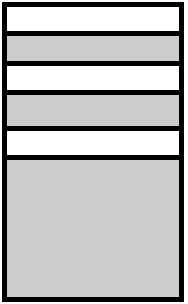
\includegraphics[width=22\unitlength]{leftlistmorem}}
% \cell{10}{35.2}{c}{\pmaxcolor$\pmax$}
% \cell{10}{28.9}{c}{\pcolor$\p$}
% \cell{10}{22.0}{c}{\pprimecolor$\p\scriptstyle'$}
\cell{10}{37.3}{c}{$\pmax$}
\cell{10}{30.5}{c}{$\p$}
\cell{10}{22.7}{c}{$\p'$}
\cell{40}{0}{b}{$q = 2$}
\cell{40}{4}{b}{\includegraphics[width=22\unitlength]{rightlistmorem}}
% \cell{40}{35.2}{c}{\pmaxcolor$\pmax$}
% \cell{40}{26.5}{c}{\pprimecolor$\p\scriptstyle'$}
% \cell{40}{14.5}{c}{\pcolor$\p$}
\cell{40}{37.3}{c}{$\pmax$}
\cell{40}{27.6}{c}{$\p'$}
\cell{40}{14.5}{c}{$\p$}
\end{picture}%
%
\hspace*{9\unitlength}%
%
\begin{picture}(60,37)
\cell{30}{-2}{t}{(b)}
% \cell{30}{5}{b}{\includegraphics[width=60\unitlength]{profile_triple_cols}}
\cell{30}{5}{b}{\includegraphics[width=60\unitlength]{profile_triple_bw}}
\cell{1}{15}{r}{$D_q^Z$}
\cell{30}{5}{t}{$q$}
% \cell{10}{18.5}{c}{\pcolor$\p$}
% \cell{6}{14}{c}{\pprimecolor$\p\scriptstyle'$}
% \cell{16}{23}{c}{\pmaxcolor$\pmax$}
\cell{10}{18.5}{c}{$\p$}
\cell{6}{14}{c}{$\p'$}
\cell{16}{23}{c}{$\pmax$}
\end{picture}
\end{center}
\caption{Visualizations of Theorem~\ref{thm:max}: (a)~in terms of how
  different values of $q$ rank the set of distributions, and (b)~in terms
  of diversity profiles.}
\lbl{fig:max-vis}
\end{figure}

Associated with the matrix $Z$ is a real number: the constant value
of any maximizing distribution.

\begin{defn}
The \demph{maximum%
%
\index{maximum diversity!matrix@of matrix} 
% 
diversity} of the matrix $Z$ is \ntn{Dmax}$\Dmax{Z} =
\sup_{\p \in \Delta_n} D_q^Z(\p)$, for any $q \in [0, \infty]$.
\end{defn}

By Theorem~\ref{thm:max}\bref{part:max-value}, $\Dmax{Z}$ is independent of
$q$. 

Later, we will see how to compute the maximizing distributions and maximum
diversity of a matrix.  For now, we just note a trivial example:

\begin{example}
\lbl{eg:max-I} 
Let $Z$ be the $n \times n$ identity matrix $I$.  We have already seen that
$D_q^I(\p) = D_q(\p)$ is maximized when $\p$ is the uniform
distribution $\vc{u}_n$, and that the maximum value is $n$
(Lemma~\ref{lemma:div-max-min}\bref{part:div-max}).  It is a special case
of Theorem~\ref{thm:max}\bref{part:max-value} that this maximum value, $n$,
is independent of $q$.  In the notation just introduced, $\Dmax{I} = n$.
\end{example}

If a distribution $\p$ maximizes diversity of order $2$, must it also
maximize diversity of orders $1$ and $\infty$, for instance?  The answer
turns out to be yes:

\begin{cor}
\lbl{cor:irrelevance}
Let $\p \in \Delta_n$.  If $\p$ maximizes $D_q^Z$ for some $q \in (0,
\infty]$ then $\p$ maximizes $D_q^Z$ for all $q \in [0, \infty]$.
\end{cor}

\begin{proof}
This is Corollary~2 of~\cite{MDBB}.
\end{proof}

The significance of this result is that if we wish to find a distribution
that maximizes diversity of all orders $q$, all we need to do is to find
one that maximizes diversity of whichever nonzero order is most convenient.

The hypothesis that $q > 0$ cannot be dropped from
Corollary~\ref{cor:irrelevance}.  Indeed, take $Z = I$.  Then $D_0^I(\p)$
is species richness%
%
\index{species!richness} 
% 
(the cardinality of $\supp(\p)$), which is maximized by any distribution
$\p$ of full support.  On the other hand, when $q > 0$, the diversity
$D_q^I(\p) = D_q(\p)$ is maximized only when $\p$ is uniform
(Lemma~\ref{lemma:div-max-min}\bref{part:div-max}).

\begin{remark}
Since the similarity-sensitive R\'enyi entropy $H_q^Z$ and
similarity-sensitive $q$-logarithmic entropy $S_q^Z$ are increasing
transformations of $D_q^Z$, the same distributions that maximize $D_q^Z$
for all $q$ also maximize $H_q^Z$ and $S_q^Z$ for all $q$.  And since
$H_q^Z = \log D_q^Z$, the maximum similarity-sensitive R\'enyi entropy,
$\sup_\p H_q^Z(\p)$, is also independent of $q$: it is simply $\log
\Dmax{Z}$.

In contrast, the maximum similarity-sensitive $q$-logarithmic entropy,
$\sup_\p S_q^Z(\p)$, is \emph{not} independent of $q$.  It is $\ln_q
\Dmax{Z}$, which varies with $q$.  This is one advantage%
% 
\index{q-logarithmic entropy@$q$-logarithmic entropy!Renyi entropy@and R\'enyi entropy}%
\index{Renyi entropy@R\'enyi entropy!q-logarithmic entropy@and $q$-logarithmic entropy}
% 
of the R\'enyi entropy (and its exponential) over the $q$-logarithmic
entropy.
\end{remark}

Theorem~\ref{thm:max} guarantees the existence of a maximizing distribution
$\pmax$, but does not tell us how to find one.  It also states that
$D_q^Z(\pmax)$ is independent of $q$, but does not tell us its value.  Our
next theorem repairs both omissions.  To state it, we need some definitions.

\begin{defn}
\lbl{defn:wtg}
A \dmph{weighting} on a matrix $M$ is a column vector $\vc{w}$ such
that $M\vc{w} = \begin{pmatrix}
  1\\ \vdots\\ 1 \end{pmatrix}$.
\end{defn}

\begin{lemma}
\lbl{lemma:wtg-cowtg}
Let $M$ be a matrix.  Suppose that $M$ and its transpose $M^\transp$
each have at least one weighting.  Then $\sum_i w_i$ is independent of the
choice of weighting $\vc{w}$ on $M$.
\end{lemma}

\begin{proof}
Let $\vc{w}$ and $\vc{w}'$ be weightings on $M$.  Choose a weighting $\vc{v}$
on $M^\transp$.  Then
\[
\sum_i w_i 
= 
(1 \ \cdots\ 1) \vc{w}
=
\bigl(M^\transp \vc{v}\bigr)^\transp \vc{w} 
=
\vc{v}^\transp M \vc{w}
=
\vc{v}^\transp \begin{pmatrix} 1\\ \vdots\\ 1 \end{pmatrix}
=
\sum_j v_j.
\]
Similarly, $\sum_i w'_i = \sum_j v_j$.  Hence $\sum_i w_i = \sum_i w'_i$.
\end{proof}

\begin{defn}
\lbl{defn:mag}
% 
Let $M$ be a matrix such that both $M$ and $M^\transp$ have at least
one weighting.  Its \demph{magnitude}%
% 
\index{magnitude!matrix@of matrix} 
% 
$\mg{M}$\ntn{magmx} is $\sum_i w_i$, where $\vc{w}$ is any weighting on
$M$.
\end{defn}

By Lemma~\ref{lemma:wtg-cowtg}, the magnitude is independent of the choice
of weighting.  

\begin{remarks}
\lbl{rmks:defn-mag}
\begin{enumerate}
\item
\lbl{rmk:defn-mag-sym}
When $M$ is symmetric (the case of interest here), $\mg{M}$ is defined as
long as $M$ has at least one weighting.  

\item
\lbl{rmk:defn-mag-inv}
When $M$ is invertible, $M$ has exactly one weighting. Its entries are
the row-sums of $M^{-1}$.  Thus, $\mg{M}$ is the sum of all the entries of
$M^{-1}$.
\end{enumerate}
\end{remarks}

\begin{defn}
A vector $\vc{v} = (v_i)$ over $\R$ is
\demph{nonnegative}%
%
\index{vector!nonnegative}% 
\index{nonnegative vector}
% 
if $v_i \geq 0$ for all $i$, and \demph{positive}%
%
\index{vector!positive}%
\index{positive!vector} 
% 
if $v_i > 0$ for all $i$.  
\end{defn}

For a nonempty subset $B \sub \{1, \ldots, n\}$, let $Z_B$\ntn{ZB} denote
the submatrix $(Z_{ij})_{i, j \in B}$ of $Z$.  This is also a symmetric
similarity matrix.  Suppose that we have a nonnegative weighting $\vc{w}$
on $Z_B$.  Then $\vc{w} \neq \vc{0}$, so $\sum_{j \in B} w_j \neq 0$.  We
can therefore define a probability distribution $\pext{\vc{w}}\ntn{pext} \in
\Delta_n$ by normalizing and extending by $0$:
\[
\pext{w}_i
% (\pext{\vc{w}})_i 
=
\begin{cases}
w_i/\mg{Z_B}      &\text{if } i \in B,    \\
0               &\text{otherwise}
\end{cases}
\]
($i \in \{1, \ldots, n\}$).  

\begin{thm}[Computation of maximum diversity]
\lbl{thm:max-comp}%
\index{maximum diversity!computation of}%
\index{magnitude!maximum diversity@vs.\ maximum diversity}%
\index{maximum diversity!magnitude@vs.\ magnitude}
% 
\begin{enumerate}
\item 
\lbl{part:max-comp-value}
The maximum diversity of $Z$ is given by
% 
\begin{equation}
\lbl{eq:comp-val}
\Dmax{Z}
=
\max_B \mg{Z_B},
\end{equation}
% 
where the maximum is over all nonempty $B \sub \{1, \ldots, n\}$ such that
$Z_B$ admits a nonnegative weighting.

\item
\lbl{part:max-comp-dist}
The set of maximizing distributions is
\[
\bigcup_B \{ 
\pext{\vc{w}} \such
\text{nonnegative weightings } \vc{w} \text{ on } B
\},
\]
where the union is over all $B$ attaining the maximum
in~\eqref{eq:comp-val}. 
\end{enumerate}
\end{thm}

\begin{proof}
This is Theorem~2 of~\cite{MDBB}.
\end{proof}

\begin{remark}
Let $B \sub \{1, \ldots, n\}$ be a subset attaining the maximum
in~\eqref{eq:comp-val}, and let $\vc{w}$ be a nonnegative weighting on
$Z_B$, so that $\pext{\vc{w}} \in \Delta_n$ is a maximizing distribution.
A short calculation shows that
\[
(Z\pext{\vc{w}})_i = \frac{1}{\mg{Z_B}}
\]
for all $i \in B$.  In particular, $(Z\pext{\vc{w}})_i$ is constant over $i
\in B$.  This can be understood as follows.  For the Hill numbers (the case
$Z = I$), the maximizing distribution takes the relative
abundances $p_i$ to be the same for all species $i$.  This is no longer
true when inter-species similarities are taken into account.  Instead, the
maximizing distributions have the property that the
\emph{ordinariness}\index{ordinariness} $(Z\p)_i$ is the same for all
species $i$ that are present.  

Determining which species are present%
%
\index{maximum diversity!elimination of species@and elimination of species}%
\index{elimination of species}%
\index{species!elimination of}
%
in a maximizing distribution is
not straightforward.  In particular, maximizing distributions do not always
have full support, a phenomenon discussed at the end of this section.
\end{remark}

Theorem~\ref{thm:max-comp} provides a finite-time algorithm for computing
the maximizing diversity of $Z$, as well as all its maximizing
distributions, as follows.

For each of the $2^n - 1$ nonempty subsets $B$ of $\{1, \ldots, n\}$,
perform some simple linear algebra to find the space of nonnegative
weightings on $Z_B$.  If this space is nonempty, call $B$ \demph{feasible}
and record the magnitude $\mg{Z_B}$.  Then $\Dmax{Z}$ is the maximum of all
the recorded magnitudes.  For each feasible $B$ such that $\mg{Z_B} =
\Dmax{Z}$, and each nonnegative weighting $\vc{w}$ on $Z_B$, the
distribution $\pext{\vc{w}}$ is maximizing.  This generates all of the
maximizing distributions.

This algorithm takes exponentially many steps in $n$, and
Remark~\ref{rmk:no-quick-clique} provides strong evidence that no algorithm
can compute maximum diversity in polynomial time.  But the situation is not
as hopeless as it might appear, for two reasons.

First, each step of the algorithm is fast, consisting as it does of solving
a system of linear equations.  For instance, using a standard laptop and a
standard computer algebra package, with no attempt at optimization, the
maximizing distributions of $25 \times 25$ matrices were computed in a few
seconds.  Second, for certain classes of matrices $Z$, the computing time
can be reduced dramatically, as we will see.

We first consider some examples, starting with the most simple cases.

\begin{example}
\lbl{eg:max-specific-two}
Take a $2 \times 2$ similarity matrix
\[
Z = 
\begin{pmatrix}
1       &z      \\
z       &1
\end{pmatrix},
\]
where $0 \leq z < 1$.  Let us run the algorithm just described.
% 
\begin{itemize}
\item
First we determine for which nonempty $B \sub \{1, \ldots, n\}$ the submatrix
$Z_B$ has a nonnegative weighting, and record the magnitudes of those that
do.  

When $B = \{1\}$, the submatrix $Z_B$ is $(1)$; this has a unique
nonnegative weighting $\vc{w} = (1)$, so $\mg{Z_B} = 1$.  The same is true
for $B = \{2\}$.  When $B = \{1, 2\}$, we have $Z_B = Z$, which has a
unique nonnegative weighting 
% 
\begin{equation}
\lbl{eq:2-wtg}
\vc{w} = \frac{1}{1 + z} \begin{pmatrix} 1\\ 1 \end{pmatrix}
\end{equation}
% 
and magnitude $\mg{Z_B} = 2/(1 + z)$.  

\item
The maximum diversity of $Z$ is given by 
\[
\Dmax{Z} 
= 
\max\Biggl\{ 1, 1, \frac{2}{1 + z} \Biggr\}, 
\]
and $2/(1 + z) > 1$, so $\Dmax{Z} = 2/(1 + z)$.  The unique
maximizing distribution is the normalization of the
weighting~\eqref{eq:2-wtg}, which is the uniform distribution $\vc{u}_2$.
\end{itemize}
% 
That the maximizing distribution is uniform conforms to the intuitive
expectation of Example~\ref{egs:max-informal}.  The computed value of
$\Dmax{Z}$ also conforms to the expectation that the maximum diversity
should be a decreasing function of the similarity between the species.
\end{example}

\begin{example}
\lbl{eg:max-specific-pond}
Now consider the three-species pond community of
Example~\ref{egs:max-informal}, with similarities as shown in
Figure~\ref{fig:pond}.  Implementing the algorithm or using
Proposition~\ref{propn:max-psd} below reveals that the unique maximizing
distribution is $(0.478, 0.261, 0.261)$
% , and the maximum diversity is $1.456$ 
(to $3$ decimal places).  This confirms the intuitive guess of
Example~\ref{egs:max-informal}.

\begin{figure}
\begin{center}
\lengths
\begin{picture}(120,16)(0,-1)
\cell{0}{7}{l}{%
$Z 
= 
\begin{pmatrix} 
1       &0.9    &0.4    \\
0.9     &1      &0.4    \\
0.4     &0.4    &1
\end{pmatrix}$}
% 
\thicklines
\put(41,-1.5){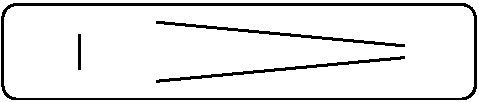
\includegraphics[width=80\unitlength]{species_triangle}}
% 
\cell{114}{7}{c}{newt}
\cell{66}{12}{r}{frog species A}
\cell{66}{2}{r}{frog species B}
% 
\cell{49}{7}{l}{0.9}
\cell{89}{12}{c}{0.4}
\cell{89}{1.7}{c}{0.4}
\end{picture}%
% }
\end{center}
\caption{Hypothetical three-species system.  Distances between species
  indicate degrees of dissimilarity between them (not to scale).}
\lbl{fig:pond}
\end{figure}
\end{example}

One of our standing hypotheses on $Z$ is symmetry.  Without it,
the main theorem fails in every respect:

\begin{example}
\lbl{eg:nonsym}
\index{symmetric!similarity matrix}
\index{similarity!matrix!nonsymmetric}
\index{maximum diversity!nonsymmetric similarity@with nonsymmetric similarity}
% 
Let $Z = \Bigl( \begin{smallmatrix} 1 & 1/2 \\ 0 & 1 \end{smallmatrix}
\Bigr)$, which is a similarity matrix but not symmetric.  Consider a
distribution $\p = (p_1, p_2) \in \Delta_2$.  If $\p$ is $(1, 0)$ or $(0,
1)$ then $D_q^Z(\p) = 1$ for all $q$.  Otherwise,
% 
\begin{align}
D_0^Z(\p)       &
=
3 - \frac{2}{1 + p_1},  
\lbl{eq:nonsym-0}
\\
D_2^Z(\p)       &
=
\frac{2}{3(p_1 - 1/2)^2 + 5/4}, 
\lbl{eq:nonsym-2}
\\
D_\infty^Z(\p)  &
=
\begin{cases}
\frac{1}{1 - p_1}       & 
\text{if } p_1 \leq 1/3,\\[.5ex]
\frac{2}{1 + p_1}       &
\text{if } p_1 \geq 1/3.
\end{cases}
\lbl{eq:nonsym-infty}
\end{align}
% 
It follows 
% from~\eqref{eq:nonsym-0} 
that $\sup_{\p \in \Delta_2} D_0^Z(\p) = 2$.  However, no distribution
maximizes $D_0^Z$; we have $D_0^Z(\p) \to 2$ as $\p \to (1, 0)$, but
$D_0^Z(1, 0) = 1$.  Equations~\eqref{eq:nonsym-2}
and~\eqref{eq:nonsym-infty} imply that
\[
\sup_{\p \in \Delta_2} D_2^Z(\p) = 1.6,
\qquad
\sup_{\p \in \Delta_2} D_\infty^Z(\p) = 1.5,
\]
with unique maximizing distributions $(1/2, 1/2)$ and $(1/3, 2/3)$
respectively.

Thus, when $Z$ is not symmetric, the main theorem fails comprehensively:
the supremum $\sup_{\p \in \Delta_n} D_0^Z(\p)$ may not be attained; there
may be no distribution maximizing $\sup_{\p \in \Delta_n} D_q^Z(\p)$ for
all $q$ simultaneously; and that supremum may vary with $q$.
\end{example}

Perhaps surprisingly, nonsymmetric similarity matrices $Z$ do have
practical uses.  For example, it is shown in Proposition~A7 of the appendix
to Leinster and Cobbold~\cite{MDISS} that the mean phylogenetic diversity
measures of Chao,%
%
\index{Chao, Anne!Chiu--Jost@--Chiu--Jost phylogenetic diversity}
%
Chiu and Jost~\cite{CCJ} are a special case of the measures $D_q^Z(\p)$,
obtained by taking a particular $Z$ constructed from the phylogenetic tree
concerned.  This $Z$ is usually nonsymmetric, reflecting the asymmetry of
evolutionary time.  More generally, the case for dropping the symmetry
axiom for metric%
%
\index{metric!nonsymmetric} 
% 
spaces was made by Lawvere%
%
\index{Lawvere, F. William} 
% 
(p.~138--139 of~\cite{LawvMSG}), and Gromov%
%
\index{Gromov, Misha} 
%
has argued that symmetry `unpleasantly limits many applications' (p.~xv
of~\cite{GromMSR}).  So, the fact that the maximum diversity theorem fails
for nonsymmetric $Z$ is an important restriction.

Now consider finite, undirected graphs with no multiple edges (henceforth,
\demph{graphs}%
%
\index{graph!maximum diversity of} 
% 
for short).  As in Example~\ref{eg:sim-matrix-gph}, any such graph
corresponds to a symmetric similarity matrix.  What, then, is the maximum
diversity of the adjacency matrix of a graph?

The answer requires some terminology.  Recall that vertices $x$ and $y$ of
a graph are said to be adjacent, written as $x \adjc y$, if there
is an edge between them.  (In particular, every vertex of a reflexive graph
is adjacent to itself.)  A set of vertices is \demph{independent}%
% 
\index{independent!set of vertices in graph} 
% 
if no two distinct vertices are adjacent.  The \demph{independence%
%
\index{independence!number}
% 
number} $\alpha(G)$\ntn{indnum} of a graph $G$ is the number of vertices in
an independent set of greatest cardinality.

\begin{propn}
\lbl{propn:graph-main}
Let $G$ be a reflexive graph with adjacency matrix $Z$.  Then the maximum
diversity $\Dmax{Z}$ is equal to the independence number $\alpha(G)$.
\end{propn}

\begin{proof}
We will maximize the diversity of order $\infty$.  For any probability
distribution $\p$ on the vertex-set $\{1, \ldots, n\}$, 
% 
\begin{equation}
\lbl{eq:graph-infty}
D_{\infty}^Z(\p)
=
1 \biggl/
\max_{i \in \supp(\p)} \sum_{j \csuch \adjco{i}{j}} p_j.
\end{equation}

First we show that $\Dmax{Z} \geq \alpha(G)$.  Choose an independent set
$B$ of cardinality $\alpha(G)$, and define $\p \in \Delta_n$ by
\[
p_i
=
\begin{cases}
1/\alpha(G)     &\text{if } i \in B,    \\
0               &\text{otherwise}.
\end{cases}
\]
For each $i \in \supp(\p) = B$, the sum on the right-hand side of
equation~\eqref{eq:graph-infty} is $1/\alpha(G)$.  Hence
$D_{\infty}^Z(\p) = \alpha(G)$, giving $\Dmax{Z} \geq \alpha(G)$.

Now we show that $\Dmax{Z} \leq \alpha(G)$.  By
equation~\eqref{eq:graph-infty}, an equivalent statement is that
for each $\p \in \Delta_n$, there is some $i \in \supp(\p)$ such that
% 
\begin{equation}
\lbl{eq:gph-max-ind}
\sum_{j \csuch \adjco{i}{j}} p_j
\geq
\frac{1}{\alpha(G)}.
\end{equation}
% 
Let $\p \in \Delta_n$.  Choose an independent
set $B \sub \supp(\p)$ with maximal cardinality among all independent
subsets of $\supp(\p)$.  Then every vertex in $\supp(\p)$ is adjacent to at
least one vertex in $B$, otherwise we could adjoin it to $B$ to make a
larger independent subset.  This gives the inequality
\[
\sum_{\,i \in B\,} \sum_{j \csuch \adjco{i}{j}} p_j
=
\sum_{\,i \in B\,} \sum_{j \in \supp(\p) \csuch \adjco{i}{j}} p_j
\geq
\sum_{j \in \supp(\p)} p_j
=
1.
\]
So we can choose some $i \in B$ such that $\sum_{j \csuch \adjco{i}{j}} p_j
\geq 1/\# B$, where $\#$ denotes cardinality.  But $\# B \leq
\alpha(G)$ since $B$ is independent, so the desired
inequality~\eqref{eq:gph-max-ind} follows.
\end{proof}

\begin{remark}
\lbl{rmk:graph-proof} 
\index{maximum diversity!elimination of species@and elimination of species}%
\index{elimination of species}%
\index{species!elimination of}
% 
The first part of the proof (together with Corollary~\ref{cor:irrelevance})
shows that a maximizing distribution on a reflexive graph can be constructed by
taking the uniform distribution on some independent set of greatest
cardinality, then extending by zero to the whole vertex-set.  Except in the
trivial case of a graph with no edges between distinct vertices, this
maximizing distribution never has full support.
\end{remark}

\begin{example}
\lbl{eg:graph-lin3}
The reflexive graph $G =
\mbox{\ensuremath{\bullet\gedge\bullet\gedge\bullet}}$ (loops not shown) has
adjacency matrix $Z = \biggl( \begin{smallmatrix} 1 &1 &0 \\ 1& 1& 1 \\ 0&
  1& 1 \end{smallmatrix} \biggr)$.  The independence number of $G$ is $2$;
this, then, is the maximum diversity of $Z$.  There is a unique
independent set of cardinality $2$, and a unique maximizing distribution,
$(1/2, 0, 1/2)$.
\end{example}

\begin{example}
\lbl{eg:graph-lin4}
The reflexive graph
$\mbox{\ensuremath{\bullet\gedge\bullet\gedge\bullet\gedge\bullet}}$ also has
independence number $2$.  There are three independent sets of maximal
cardinality, so by Remark~\ref{rmk:graph-proof}, there are at least three
maximizing distributions,
\[
\bigl(\hlf, 0, \hlf, 0\bigr),
\qquad
\bigl(\hlf, 0, 0, \hlf\bigr),
\qquad
\bigl(0, \hlf, 0, \hlf\bigr),
\]
all with different supports.  (The possibility of multiple maximizing
distributions was also observed in the case $q = 2$ by Pavoine and
Bonsall~\cite{PaBo}.)
% 
In fact, there are further maximizing distributions not constructed in the
proof of Proposition~\ref{propn:graph-main}, namely, $\bigl(\hlf, 0, t,
\hlf - t\bigr)$ and $\bigl(\hlf - t, t, 0, \hlf\bigr)$ for all $t \in (0,
\hlf)$.
\end{example}

\begin{example}
Kolmogorov's notion of the $\epsln$-entropy of a metric
space~\cite{KolmCAC} is approximately an instance of maximum diversity,
assuming that one is interested in its behaviour as $\epsln \to 0$ rather
than for individual values of $\epsln$.

Let $A$ be a finite metric space.  Given $\epsln > 0$, the
\demph{$\epsln$-covering%
%
\index{covering number} 
% 
number} $N_\epsln(A)$ is the smallest number of closed $\epsln$-balls
needed to cover $A$.  But also associated with $\epsln$ is the graph%
%
\index{graph!maximum diversity of} 
% 
$G_\epsln(A)$ whose vertices are the points of $A$ and with an edge between
$a$ and $b$ whenever $d(a, b) \leq \epsln$.  Write $Z_\epsln(A)$ for the
adjacency matrix of $G_\epsln(A)$.  From
Proposition~\ref{propn:graph-main}, it is not hard to deduce that
\[
N_\epsln(A) \leq \Dmax{Z_\epsln(A)} \leq N_{\epsln/2}(A)
\]
(Example~11 of~\cite{MDBB}).  

We have repeatedly seen that quantities called entropy tend to be the
logarithms of quantities called diversity.  Kolmogorov's
\demph{$\epsln$-entropy}%
% 
\index{entropy!Kolmogorov}%
\index{Kolmogorov, Andrei!entropy}%
\index{metric!entropy} 
% 
of $A$ is $\log N_\epsln(A)$, and, by the inequalities above, is closely
related to the logarithm of maximum diversity.
\end{example}

The moral of the proof of Proposition~\ref{propn:graph-main} is that by
performing the simple task of maximizing diversity of order $\infty$, we
automatically maximize diversity of all other orders.  Here is an example
of how this observation can be exploited.

Every graph $G$ has a \dmph{complement} $\gcomp{G}$, with the same
vertex-set as $G$; two vertices are adjacent in $\gcomp{G}$ if and only if
they are not adjacent in $G$.  Thus, the complement of a reflexive graph is
\demph{irreflexive}%
%
\index{irreflexive}%
\index{graph!irreflexive} 
% 
(has no loops), and vice versa.  A set $B$ of vertices
in an irreflexive graph $X$ is a \dmph{clique} if all pairs of distinct
elements of $B$ are adjacent in $X$.  The \demph{clique
number} \ntn{clinum}$\cliqueno{X}$ of $X$ is the maximal cardinality of a
clique in $X$.  Thus, $\cliqueno{X} = \alpha\bigl(\gcomp{X}\bigr)$.

We now recover a result of Berarducci, Majer and Novaga (Proposition~5.10
of~\cite{BMN}).

\begin{cor}[Berarducci, Majer and Novaga]
\index{Berarducci, Alessandro}%
\index{Majer, Pietro}%
\index{Novaga, Matteo}%
% \lbl{cor:graph-capacity}
% 
Let $X$ be an irreflexive graph.  Then
\[
\sup_\p \sum_{(i, j) \csuch \adjco{i}{j}} p_i p_j
=
1 - \frac{1}{\cliqueno{X}},
\]
where the supremum is over probability distributions $\p$ on the vertex-set
of $X$ and the sum is over ordered pairs of adjacent vertices of $X$.
\end{cor}

\begin{proof}
Write $\{1, \ldots, n\}$ for the vertex-set of $X$, and $Z$ for the
adjacency matrix of the reflexive graph $\gcomp{X}$.  Then for all $\p \in
\Delta_n$, 
% 
\begin{align*}
\sum_{(i, j) \csuch \adjcoin{i}{j}{X}} p_i p_j        &
=
\sum_{i, j = 1}^n p_i p_j - 
\sum_{(i, j) \csuch \adjcoin{i}{j}{\gcomp{X}}} p_i p_j  \\
&
=
1 - \sum_{i, j = 1}^n p_i Z_{ij} p_j    \\
&
=
1 - \frac{1}{D_2^Z(\p)}.
\end{align*}%
% 
Hence by Proposition~\ref{propn:graph-main},
\[
\sup_{\p \in \Delta_n} \sum_{(i, j) \csuch \adjcoin{i}{j}{X}} p_i p_j    
=
1 - \frac{1}{\Dmax{\p}}
= 
1 - \frac{1}{\alpha\bigl(\gcomp{X}\bigr)}
=
1 - \frac{1}{\cliqueno{X}}.
\]
\end{proof}

It follows from this proof and Remark~\ref{rmk:graph-proof} that $\sum_{(i,
  j)\csuch \adjco{i}{j}} p_i p_j$ can be maximized as follows: take the
uniform distribution on some clique in $X$ of maximal cardinality, then
extend by zero to the whole vertex-set.  This distribution maximizes the
probability that two vertices chosen at random are adjacent, as in
Example~\ref{egs:dqz}\bref{eg:dqz-two}. 

\begin{remark}
\lbl{rmk:no-quick-clique}
Proposition~\ref{propn:graph-main} implies that computationally, finding
the maximum diversity of an arbitrary symmetric $n \times n$ similarity
matrix is at least as hard as finding the independence number of a
reflexive graph with $n$ vertices.  This is a very well-studied problem,
usually presented in its dual form (find the clique number of an
irreflexive graph) and called the 
\demph{maximum%
%
\index{maximum clique problem}%
\index{clique}
% 
clique problem}~\cite{Karp}.  It is $\mathbf{NP}$-hard.  Hence, assuming
that $\mathbf{P} \neq \mathbf{NP}$, there is no polynomial-time algorithm
for computing maximum diversity, nor even for computing the support of a
maximizing distribution.
\end{remark}

We now return to general symmetric similarity matrices, addressing two
remaining questions: when are maximizing distributions unique, and when do
they have full support?

Recall that a real symmetric matrix $Z$ is \demph{positive%
%
\index{positive!definite} 
% 
definite} if $\vc{x}^\transp
Z \vc{x} > 0$ for all $\vc{0} \neq \vc{x} \in \R^n$, and \demph{positive
  semidefinite}%
% 
\index{positive!semidefinite} 
% 
if $\vc{x}^\transp Z \vc{x} \geq 0$ for all $\vc{x} \in 
\R^n$.  Equivalently, $Z$ is positive definite if all its eigenvalues are
positive, and positive semidefinite if they are all nonnegative.  A
positive definite matrix is invertible and therefore has a unique weighting.

\begin{propn}
\lbl{propn:max-psd}
\begin{enumerate}
\item 
If $Z$ is positive semidefinite and has a nonnegative weighting $\vc{w}$,
then $\Dmax{Z} = \mg{Z}$ and $\vc{w}/\mg{Z}$ is a maximizing distribution.

\item
If $Z$ is positive definite and its unique weighting $\vc{w}$ is positive
then $\vc{w}/\mg{Z}$ is the unique maximizing distribution.
\end{enumerate}
\end{propn}

\begin{proof}
This is Proposition~3 of~\cite{MDBB}.
\end{proof}

In particular, if $\mg{Z}$ is positive semidefinite and has a nonnegative
weighting, then computing its maximum diversity is trivial.

When $Z$ is positive definite and its unique weighting is positive,
its unique maximizing distribution eliminates no species.  Here are two
classes of such matrices $Z$.

\begin{example}
\lbl{eg:ultra-pos-def}
% 
Call $Z$ \demph{ultrametric}\index{ultrametric!matrix} if $Z_{ik} \geq
\min\{Z_{ij}, Z_{jk}\}$ for all $i, j, k$ and $Z_{ii} > Z_{jk}$ for all $i,
j, k$ with $j \neq k$.  For instance, the matrix $Z = \bigl(e^{-d(i,
  j)}\bigr)$ of any ultrametric space is ultrametric; see
Example~\ref{eg:sim-matrix-met}.  If $Z$ is ultrametric then $Z$ is
positive definite with positive weighting, by Proposition~2.4.18 of
Leinster~\cite{MMS}.

(The positive definiteness of ultrametric matrices was also proved,
earlier, by Varga and Nabben~\cite{VaNa}, and a different proof still was
given in Theorem~3.6 of Meckes~\cite{MeckPDM}.  An earlier, indirect proof
of the positivity of the weighting can be found in Pavoine, Ollier and
Pontier~\cite{POP}.)

Such matrices arise in practice.  For instance, $Z$ is ultrametric if it is
defined from a phylogenetic or taxonomic tree as in
Examples~\ref{egs:sim}\bref{eg:sim-phylo} and~\bref{eg:sim-taxo}.  
\end{example}

\begin{example}
\lbl{eg:id-pos-def}
The identity matrix $Z = I$ is certainly positive definite with positive
weighting.  By topological arguments, there is a neighbourhood $U$ of $I$
in the space of symmetric matrices such that every matrix in $U$ also has
these properties.  (See the proofs of Propositions~2.2.6 and~2.4.6 of
Leinster~\cite{MMS}.)  

Quantitative versions of this result are also available.  For instance,
suppose that $Z_{ii} = 1$ for all $i, j$ and that $Z$ is \demph{strictly
  diagonally dominant},%
% 
\index{diagonally dominant}%
\index{strictly diagonally dominant}
% 
that is, $Z_{ii} > \sum_{j \neq i} Z_{ij}$ for all $i$.  Then $Z$ is
positive definite with positive weighting (Proposition~4 of Leinster and
Meckes~\cite{MDBB}).
\end{example}

In summary, if our similarity matrix $Z$ is ultrametric, or if it is close
to the matrix $I$ that encodes the naive model, then it enjoys many special
properties: the maximum diversity is equal to the magnitude, there is a
unique maximizing distribution, the maximizing distribution has full
support, and both the maximizing distribution and the maximum diversity can
be computed in polynomial time.

We saw in Examples~\ref{eg:graph-lin3} and~\ref{eg:graph-lin4} that for
some similarity matrices $Z$, no maximizing distribution has full
support.  Mathematically, this simply means that maximizing distributions
sometimes lie on the boundary of $\Delta_n$.  But ecologically, it may
sound shocking: is it reasonable that diversity can be increased by
\emph{eliminating} some species?%
% 
\index{maximum diversity!elimination of species@and elimination of species}%
\index{elimination of species}%
\index{species!elimination of}

We argue that it is.  For example, consider a forest%
%
\index{forest!oak and pine} 
%
consisting of one species of oak and ten species of pine, with all species
equally abundant.  Suppose that an eleventh species of pine is added, with
the same abundance as all the existing species (Figure~\ref{fig:pine}).
This makes the forest even more heavily dominated by pine than it was
before, so it is intuitively reasonable that the diversity should decrease.
But now running time backwards, the conclusion is that if we start with a
forest containing the oak and all eleven pine species, then eliminating%
% 
\index{elimination of species}%
\index{species!elimination of}
% 
the eleventh should \emph{increase} the diversity.

\begin{figure}
\centering
\lengths
\begin{picture}(120,23)
\cell{60}{-.7}{b}{\includegraphics[width=77\unitlength]{forestplus}}
\cell{29.5}{17.2}{c}{oak}
\cell{82}{20}{c}{pine}
\end{picture}
\caption{Hypothetical community consisting of one species of oak
  ($\scriptscriptstyle\blacksquare$) and ten species of pine ($\bullet$), to
  which one further species of pine is then added ($\circ$).  Distances
  between species indicate degrees of dissimilarity (not to scale).}
\lbl{fig:pine}
\end{figure}

To clarify further, recall that diversity is defined in terms of the
\emph{relative}%
%
\index{abundance!relative vs.\ absolute} 
% 
abundances only.  Thus, eliminating the $i$th species causes not only a
decrease in $p_i$, but also an increase in the other relative abundances
$p_j$.  If the $i$th species is particularly ordinary within the community
(like the eleventh species of pine), then eliminating it increases the
relative abundances of less ordinary species, resulting in a community that
is more diverse.

The instinct that maximizing diversity should not eliminate any species is
based on the assumption that the distinction between species is of high
value.  (After all, if two species were very nearly identical~-- or in the
extreme, actually identical~-- then losing one would be of little
importance.)  If one wishes to make that assumption, one must build it into
the model.  This is done by choosing a similarity%
% 
\index{similarity!matrix!choice of} 
% 
matrix $Z$ with a low similarity coefficient $Z_{ij}$ for each $i \neq j$.
Thus, $Z$ is close to the identity matrix $I$ (assuming that similarity is
measured on a scale of $0$ to $1$).  Example~\ref{eg:id-pos-def} guarantees
that in this case, there is a unique maximizing distribution and it does
not, in fact, eliminate any species.

The fact that maximizing distributions can eliminate some species has
previously been discussed in the ecological literature in the case of Rao's
quadratic entropy ($q = 2$): see Izs\'ak and Szeidl~\cite{IzSz},
Pavoine and Bonsall~\cite{PaBo}, and references therein.  The same
phenomenon was observed and explored by Shimatani in
genetics~\cite{ShimADD}, again in the case $q = 2$.

We finish by stating necessary and sufficient conditions for a symmetric
similarity matrix $Z$ to admit at least one maximizing distribution of full
support, so that diversity can be maximized without eliminating any
species.  We also state necessary and sufficient conditions for
\emph{every} maximizing distribution to have full support.  The latter
conditions are genuinely more restrictive.  For instance, if $Z =
\bigl( \begin{smallmatrix} 1& 1\\ 1& 1\\ \end{smallmatrix} \bigr)$ then
every distribution is maximizing, so some but not all maximizing
distributions have full support.

\begin{propn}
\lbl{propn:semi}
The following are equivalent:
% 
\begin{enumerate}
\item
\lbl{part:semivec}
there exists a maximizing distribution for $Z$ of full support;

\item
\lbl{part:semidef}
$Z$ is positive semidefinite and has at least one positive weighting.
\end{enumerate}
\end{propn}

\begin{proof}
This is Proposition~5 of~\cite{MDBB}.
\end{proof}


\begin{propn}
The following are equivalent:
% 
\begin{enumerate}
\item
\lbl{part:vec}
every maximizing distribution for $Z$ has full support;

\item
\lbl{part:unique}
$Z$ has exactly one maximizing distribution, which has full support;

\item
\lbl{part:def}
$Z$ is positive definite with positive weighting;

\item 
\lbl{part:crit}
$\Dmax{Z_B} < \Dmax{Z}$ for every nonempty proper subset $B$ of $\{1,
  \ldots, n\}$.
\end{enumerate}
\end{propn}

\begin{proof}
This is Proposition~6 of~\cite{MDBB}.
\end{proof}

Let us put our results on maximum diversity into context.  First, they
belong to the huge body of work on maximum entropy.  For example,
among all probability distributions on $\R$ with a given mean and variance,
the one with the maximum% 
% 
\index{maximum entropy}
% 
entropy is the normal%
%
\index{normal distribution} 
% 
distribution~\cite{LinnITP,BarrECL}.  Given the
fundamental nature of the normal distribution, this fact alone would
be motivation enough to seek maximum entropy distributions in other
settings (such as the one at hand), quite apart from the importance of
maximum entropy in thermodynamics, machine learning, and so on.

Second, the maximum diversity theorem (Theorem~\ref{thm:max}) is stated for
probability distributions on \emph{finite} sets equipped with a similarity
matrix, but it can be generalized to compact Hausdorff spaces $A$ equipped
with a suitable function $Z \from A \times A \to [0, \infty)$ measuring
similarity between points.  This more general theorem was recently proved
by Leinster and Roff~\cite{MEMS},%
%
\index{Roff, Emily}%
\index{entropy!metric space@on metric space}%
\index{maximum diversity!theorem}
%
along with a version of the computation theorem
(Theorem~\ref{thm:max-comp}).  It encompasses both the finite case and the
case of a compact metric space with similarities $Z(a, b) = e^{-d(a, b)}$.

Third, maximum diversity is closely related to the emerging invariant
known as magnitude, as now described.
\index{Meckes, Mark|)}


\section{Introduction to magnitude}
\lbl{sec:mag}
\index{magnitude}


In the solution to the maximum diversity problem, a supporting role was
played by the notion of the magnitude of a matrix
(Definition~\ref{defn:mag}).  Theorem~\ref{thm:max-comp} implies that the
maximum diversity of a symmetric similarity matrix $Z$ is always equal to
the magnitude of one of its principal submatrices $Z_B$, and
Examples~\ref{eg:ultra-pos-def} and~\ref{eg:id-pos-def} describe classes of
matrix for which the maximum diversity is actually equal to the magnitude.

The definition of magnitude was introduced without motivation, and may
appear to be nothing but a technicality.  But in fact, magnitude is
an answer to the following very broad conceptual challenge.

For many types of objects in mathematics, there is a canonical notion of
size.\index{size}  For example:
% 
\begin{itemize}
\item 
Every set $A$ (finite, say) has a cardinality\index{cardinality} $\mg{A}$,
which satisfies the 
inclusion-exclusion%
%
\index{inclusion-exclusion principle} 
%
formula
\[
\mg{A \cup B} = \mg{A} + \mg{B} - \mg{A \cap B}
\]
(for subsets $A$ and $B$ of some larger set) and the
multiplicativity%
%
\index{multiplicative!cardinality is} 
% 
formula 
\[
\mg{A \times B} = \mg{A} \cdot \mg{B}.
\]

\item 
Every measurable subset $A$ of Euclidean space has a volume\index{volume}
$\Vol(A)$, which satisfies similar formulas:
% 
\begin{align*}
\Vol(A \cup B)  &
= 
\Vol(A) + \Vol(B) - \Vol(A \cap B),   \\
\Vol(A \times B)        & 
= 
\Vol(A) \cdot \Vol(B).
\end{align*}

\item 
Every sufficiently well-behaved topological space $A$ has an Euler
characteristic%
%
\index{Euler characteristic}
%
$\chi(A)$\ntn{ECsp}, which again satisfies
% 
\begin{align*}
\chi(A \cup B)  & 
= 
\chi(A) + \chi(B) - \chi(A \cap B),   \\
\chi(A \times B)        &
=
\chi(A) \cdot \chi(B).
\end{align*}
% 
(Here, inclusion-exclusion holds for subspaces $A$ and $B$ of some larger
space, under suitable hypotheses.  Technically, it is best to work
in the setting of either cohomology with compact supports, as in
Section~3.3 of Hatcher~\cite{Hatc}, or tame topology, as in Chapter~4 of
van den Dries~\cite{VDD} or Chapter~3 of Ghrist~\cite{GhriEAT}.)  The
insight that Euler%
%
\index{Euler characteristic} 
% 
characteristic is the topological analogue of cardinality is
principally due to Schanuel, who compared Euler's investigation of spaces
of negative `cardinality' (Euler characteristic) with Cantor's
investigation of sets of infinite cardinality:
% 
\begin{quote}
\index{Schanuel, Stephen}
% 
Euler's analysis, which demonstrated that in counting suitably `finite'
spaces%
%
\index{set theory} 
% 
one can get well-defined negative integers, was a revolutionary advance in
the idea of cardinal number~-- perhaps even more important than Cantor's
extension to infinite sets, if we judge by the number of areas in
mathematics where the impact is pervasive.
\end{quote}
% 
(\cite{SchaNSE}, Section~3).
\end{itemize}

The close resemblance between these invariants suggests a challenge: find a
general notion of the size of a mathematical object, encompassing these
three invariants and others.  And this challenge has a solution: the
magnitude of an enriched category.%
%
\index{category theory}

Enriched categories are very general structures, and the theory of the
magnitude of an enriched category sweeps across many parts of mathematics,
most of them very distant from diversity measurement.  This section and the
next paint a broad-brush picture, omitting all details.  General references
for this material are Leinster and Meckes~\cite{MMSCG} and
Leinster~\cite{MMS}.

We begin with ordinary categories.  A finite category\index{category}
$\scat{A}$ consists of, first of all, a finite directed multigraph, that is,
a finite collection of objects $a_1, \ldots, a_n$ together with a finite
set $\Hom(a_i, a_j)$ for each $i$ and $j$, whose elements are to be thought
of as maps or arrows from $a_i$ to $a_j$ (Figure~\ref{fig:fin-cat}).  It is
also equipped with an associative operation of composition of maps and an
identity map on each object.  (See Mac~Lane~\cite{MacLCWM}, for instance.)

\begin{figure}
\centering
\lengths
\begin{picture}(120,23)
\cell{60}{10.5}{c}{\includegraphics[width=87\unitlength]{fincat.pdf}}
\cell{16}{2}{c}{\large$a_1$}
\cell{30}{21}{c}{\large$a_2$}
\cell{46}{2}{c}{\large$a_3$}
\cell{63}{14}{c}{\large$a_4$}
\cell{92}{10}{c}{\large$a_5$}
\end{picture}
\caption{The objects and maps of a finite category (identity maps not
  shown).}
\lbl{fig:fin-cat}
\end{figure}

Any finite category $\scat{A}$ gives rise to an $n \times n$ matrix
$Z_{\scat{A}}$ whose $(i, j)$-entry is $\mg{\Hom(a_i, a_j)}$, the number
of maps from $a_i$ to $a_j$.  The \demph{magnitude}%
% 
\index{magnitude!category@of category}
% 
$\mg{\scat{A}}\ntn{magcat} \in \Q$ of the category $\scat{A}$ is defined to
be the magnitude $\mg{Z_{\scat{A}}}$ of the matrix $Z_{\scat{A}}$, if it
exists.

Here we have used the notation $\mg{\,\cdot\,}$ for two purposes: first for
the cardinality of a finite set, then for the magnitude of a category.
This is deliberate.  In both cases, $\mg{\,\cdot\,}$ is a measure
of the size of the structure concerned.

For example, if $\scat{A}$ has no maps except for identities then
$Z_{\scat{A}}$ is the $n \times n$ identity matrix, so the magnitude
$\mg{\scat{A}}$ is the cardinality $n$ of its set of objects.  Less
trivially, any (small) category $\scat{A}$ has a classifying%
% 
\index{classifying space} 
% 
space $B\scat{A}$ (also called its nerve\index{nerve} 
or geometric%
%
\index{geometric realization} 
% 
realization), which is a topological space constructed from $\scat{A}$ by
starting with one $0$-simplex for each object of $\scat{A}$, then pasting
in one $1$-simplex for each map in $\scat{A}$, one $2$-simplex for each
commutative triangle in $\scat{A}$, and so on (Segal~\cite{SegaCSS}).  It is a
theorem that
% 
\begin{equation}
\lbl{eq:mag-classifying}
\mg{\scat{A}} = \chi(B\scat{A}),
\end{equation}
% 
under finiteness conditions to ensure that the Euler%
%
\index{Euler characteristic} 
%
characteristic of $B\scat{A}$ is well-defined
(Proposition~2.11 of Leinster~\cite{ECC}).  So, the situation is similar to
group homology\index{homology}: the homology of a group $G$ can be
defined either through a direct algebraic formula (as for $\mg{\scat{A}}$)
or as the homology of its classifying space (as for $\chi(B\scat{A})$), and
it is a theorem that the two are equal.

\begin{example}
Let $\scat{A} = (\bullet \parpairu \bullet)$ (identity maps not shown).
Then  
\[
Z_{\scat{A}} 
= 
\begin{pmatrix}
1       &2      \\
0       &1  
\end{pmatrix},
\]
giving
\[
Z_{\scat{A}}^{-1}
=
\begin{pmatrix}
1       &-2     \\
0       &1  
\end{pmatrix}
\]
and so
\[
\mg{\scat{A}}
=
\mg{Z_{\scat{A}}}
=
1 + (-2) + 0 + 1
=
0.
\]
On the other hand, $B\scat{A} = S^1$, so $\chi(B\scat{A}) = 0$,
confirming equation~\eqref{eq:mag-classifying}.
\end{example}

Equation~\eqref{eq:mag-classifying} shows how, under hypotheses, magnitude
for categories can be derived from Euler%
%
\index{Euler characteristic} 
% 
characteristic for topological spaces.  In the other direction, we can
derive topological Euler characteristic from categorical magnitude.  Let
$M$ be a finitely triangulated manifold.  Then associated with the
triangulation, there is a category $\scat{A}_M$ whose objects are the
simplices $s_1, \ldots, s_n$ of the triangulation, with one map $s_i \to
s_j$ whenever $s_i \sub s_j$, and with no maps $s_i \to s_j$ otherwise.
Then
\[
\chi(M) = \mg{\scat{A}_M}
\]
(Section~3.8 of Stanley~\cite{StanEC1} and Section~2 of
Leinster~\cite{ECC}).

The moral of the last two results is that topological Euler characteristic
and categorical magnitude each determine the other (under suitable
hypotheses).  Indeed, the magnitude of a category is often called its Euler
characteristic; see, for instance, Leinster~\cite{ECC}, Berger and
Leinster~\cite{ECCSDS}, Fiore, L\"uck and Sauer~\cite{FLSECC,FLSFOE},
Noguchi~\cite{NoguECA,NoguECC,NoguZFF}, and Tanaka~\cite{TanaECB}.

Further theorems connect the magnitude of a category to the Euler
characteristic of an orbifold (Proposition~2.12 of~\cite{ECC}) and to the
Baez--Dolan%
% 
\index{Baez, John!Dolan cardinality@--Dolan cardinality}%
\index{Dolan, James}%
\index{groupoid cardinality}%
\index{cardinality!groupoid@of groupoid}
% 
cardinality of a groupoid (Example~2.7 of~\cite{ECC} and
Section~3 of Baez and Dolan~\cite{BaDoFSF}), both of which are rational
numbers, not usually integers.  The notion of magnitude can also be seen as
an extension of the theory of M\"obius%
% 
\index{Mobius--Rota inversion@M\"obius--Rota inversion} 
% 
inversion for posets (most commonly
associated with the name of Rota~\cite{RotaFCT}),%
%
\index{Rota, Gian-Carlo}
% 
which itself generalizes the classical M\"obius function of number theory;
see~\cite{ECC,NMI} for explanation.

The definition of the magnitude of a category involved $\mg{\Hom(a_i,
  a_j)}$, the cardinality of the set of maps from $a_i$ to $a_j$.  Thus, we
used the notion of the cardinality of a finite set to define the magnitude
of a finite category.  We can envisage that if $\Hom(a_i, a_j)$ were some
other kind of structure with a preexisting notion of size, a similar
definition could be made.  And indeed, this idea can be implemented in the
language of enriched categories, as follows.

A \demph{monoidal%
%
\index{monoidal category}
% 
category} is, loosely speaking, a category $\cat{V}$ equipped with a
product operation satisfying reasonable conditions.  Section~VII.1 of
Mac~Lane~\cite{MacLCWM} gives the full definition, but the following
examples will be all that we need here.

\begin{examples}
Typical examples of monoidal categories are the category $\Set$ of sets
with the cartesian product $\times$ and the category $\Vect$ of vector
spaces with the tensor product $\otimes$.

A less obvious example is the category whose objects are the elements of
the interval $[0, \infty]$, with one map $x \to y$ whenever $x \geq y$, and
with no maps $x \to y$ otherwise.  Here we take $+$ as the `product'
operation.  (We could also take ordinary multiplication as the product, but
it is $+$ that will be of interest here.)
\end{examples}

Now fix a monoidal category $\cat{V}$, with product denoted by $\otimes$.
Loosely, a \demph{category enriched in $\cat{V}$},%
%
\index{enriched category}
%
or \demph{$\cat{V}$-category},%
%
\index{Vcategory@$\cat{V}$-category}
%
$\scat{A}$, consists of:
% 
\begin{itemize}
\item 
a set $a, b, \ldots$ of \demph{objects} of $\scat{A}$;

\item
for each pair $(a, b)$ of objects of $\scat{A}$, an object $\Hom(a, b)$ of
$\cat{V}$;

\item
for each triple $(a, b, c)$ of objects of $\scat{A}$, a map 
% 
\begin{equation}
\lbl{eq:enr-comp}
\Hom(a, b) \otimes \Hom(b, c) \to \Hom(a, c)
\end{equation}
% 
in $\cat{V}$ (called \demph{composition} in $\scat{A}$),
\end{itemize}
% 
subject to conditions.  (For the full definition, see Section~1.2 of
Kelly~\cite{KellBCE} or Section~6.2 of Borceux~\cite{BorcHCA2}.)

\begin{examples}
The following examples of enriched categories are depicted in
Figure~\ref{fig:mon-enr}.
% 
\begin{enumerate}
\item 
A category enriched in $(\Set, \times)$ is just an ordinary category.  So,
an enriched category is not a category with special properties; it is
something \emph{more general} than a category.

\item
A category enriched in $(\Vect, \otimes)$ is a 
\demph{linear%
%
\index{linear category} 
%
category}: a category equipped with a vector space structure on each of the
sets $\Hom(a, b)$, in such a way that composition is bilinear.

\item
As first observed by Lawvere~\cite{LawvMSG},%
%
\index{Lawvere, F. William} 
% 
any metric space $A$ can be viewed as a category $\scat{A}$ enriched in
$([0, \infty], +)$: the objects of $\scat{A}$ are the points of $A$, while
$\Hom(a, b) \in [0, \infty]$ is the distance $d(a, b)$, and the
composition~\bref{eq:enr-comp} is the triangle inequality
\[
d(a, b) + d(b, c) \geq d(a, c).
\]
\end{enumerate}
\end{examples}

Thus, categories, linear categories and metric spaces are all instances of
a single general concept: enriched category.  This enables constructions
and insights to be passed backwards and forwards between them, a strategy
that proves to have great power.

\begin{figure}
\centering
\lengths
\begin{picture}(120,72)(0,0)
\thicklines
\cell{30}{0}{bl}{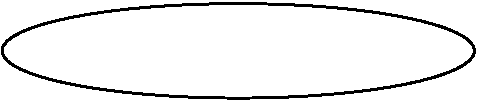
\includegraphics[width=81\unitlength]{ellipse.pdf}}
\cell{15}{11}{c}{\large monoidal}
\cell{15}{6}{c}{\large categories}
% 
\cell{40}{9}{c}{$\zmark$}
\cell{42}{9}{l}{$\cat{V}$}
% 
\cell{60}{12}{c}{$\zmark$}
\cell{62}{12}{l}{$\Set$}
% 
\cell{75}{5}{c}{$\zmark$}
\cell{77}{5}{l}{$\Vect$}
% 
\cell{95}{10}{c}{$\zmark$}
\cell{97}{10}{l}{$[0, \infty]$}
% 
\cell{30}{72}{tl}{\includegraphics[width=81\unitlength]{cylinder.pdf}}
\cell{15}{49}{c}{\large enriched}
\cell{15}{44}{c}{\large categories}
% 
\put(40,32){\line(0,1){31}}
\cell{41}{48}{l}{\rotatebox{-90}{$\cat{V}$-categories}}
% 
\put(60,35){\line(0,1){31}}
\cell{61}{51}{l}{\rotatebox{-90}{categories}}
% 
\put(75,28){\line(0,1){31}}
\cell{76}{43}{l}{\rotatebox{-90}{linear categories}}
% 
\put(95,33){\line(0,1){31}}
\cell{96}{47}{l}{\rotatebox{-90}{metric spaces}}
\end{picture}
\caption{Schematic diagram of monoidal and enriched categories.}
\lbl{fig:mon-enr}
\end{figure}

In particular, it is straightforward to generalize the definition of the
magnitude of a finite category to finite enriched categories.  Let
$\cat{V}$ be a monoidal category equipped with a function
$\mg{\,\cdot\,}$\ntn{gauge} that assigns to each object $X$ of $\cat{V}$ an
element $\mg{X}$ of some ring.  This function $\mg{\,\cdot\,}$ is to play the
role of the cardinality of a finite set, and we therefore impose the
requirements that it is isomorphism-invariant and multiplicative:
\[
X \iso Y \implies \mg{X} = \mg{Y},
\qquad
\mg{X \otimes Y} = \mg{X} \cdot \mg{Y}.
\]
(Section~1.3 of Leinster~\cite{MMS} gives details.)  Then any
$\cat{V}$-category $\scat{A}$ with finitely many objects, $a_1, \ldots,
a_n$, gives rise to a matrix
\[
Z_{\scat{A}} = \bigl( \mg{\Hom(a_i, a_j)} \bigr)_{i, j}.
\]
The \demph{magnitude}%
% 
\index{magnitude!enriched category@of enriched category} 
% 
$\mg{\scat{A}}$ of $\scat{A}$ is defined to be the magnitude of
$Z_{\scat{A}}$, if it exists.

\begin{example}
If we begin with the monoidal category $\cat{V}$ of finite sets equipped
with the cartesian product, with the cardinality function
$\mg{\mbox{\ensuremath{\,\cdot\,}}}$ on finite sets, then we recover the
notion of the magnitude of a finite category.
\end{example}

\begin{example}
Let $\cat{V}$ be the category of finite-dimensional vector spaces over some
field, with the tensor product, and put $\mg{X} = \dim X$ for
finite-dimensional vector spaces $X$.  Then we obtain a notion of the
magnitude $\mg{\scat{A}}$ of a linear category $\scat{A}$ with finitely
many objects and finite-dimensional hom-spaces $\Hom(a, b)$.  By
definition, $\mg{\scat{A}}$ is the magnitude of the matrix
\[
\bigl( \dim \Hom(a, b) \bigr)_{a, b \in \scat{A}}.
\]
For instance, let $E$ be an associative algebra%
% 
\index{associative algebra} 
% 
over an algebraically closed field.  In the representation theory of
algebras, an important linear category associated with $E$ is $\IP(E)$, the
category of indecomposable%
% 
\index{indecomposable module} 
% 
projective%
% 
\index{projective module} 
% 
$E$-modules.  Under finiteness hypotheses on $E$, it is a theorem that
$\IP(E)$ has magnitude
% 
\begin{equation}
\lbl{eq:ip}
% \[
\mg{\IP(E)} 
=
\sum_{n = 0}^\infty (-1)^n \dim \Ext_E^n(S, S),
% \]
\end{equation}
% 
where $S$ is the direct sum of the simple $E$-modules (Theorem~1.1 of
Chuang,%
%
\index{Chuang, Joseph}
%
King%
%
\index{King, Alastair} 
% 
and Leinster~\cite{MFDA}).  The
matrix $Z_{\IP(E)}$ is better known as the \demph{Cartan%
%
\index{Cartan matrix} 
% 
matrix} of $E$.  The right-hand side of equation~\eqref{eq:ip} is called
the \demph{Euler%
%
\index{Euler form} 
% 
form} $\chi(S, S)$ of the pair $(S, S)$, and is another manifestation of
the concept of Euler characteristic.
\end{example}

The examples so far of the magnitude of an enriched category have been
closely related to other, older invariants.  But when we apply the
definition to metric spaces, we obtain something new.

Let $\cat{V}$ be the monoidal category $[0, \infty]$, with product $+$.
For $x \in [0, \infty]$, define
\[
\mg{x} = e^{-x} \in \R.
\]
(Recall that $\mg{\,\cdot\,}$ is required to be `multiplicative', that is,
must convert the tensor product on $\cat{V}$ into multiplication.  In
this case, this means $\mg{x + y} = \mg{x} \cdot \mg{y}$, which by
Corollary~\ref{cor:add-transf}\bref{part:add-transf-exp} essentially forces
$\mg{x} = c^x$ for some constant $c$.)  Then we obtain a notion of the
magnitude of a finite $\cat{V}$-category, and in particular, of a finite
metric space.

In explicit terms, the definition is as follows.  Let $A = \{a_1, \ldots,
a_n\}$ be a finite metric\index{metric!space} space.  Form the $n \times n$
matrix
\[
Z_A = \bigl( e^{-d(a_i, a_j)} \bigr).
\]
Invert $Z_A$ (if possible); then the \demph{magnitude}%
% 
\index{magnitude!metric space@of metric space}
% 
$\mg{A}$ of $A$ is
the sum of all $n^2$ entries of $Z_A^{-1}$.

Here we have used Remark~\ref{rmks:defn-mag}\bref{rmk:defn-mag-inv} on the
magnitude of a matrix in terms of its inverse.  Since $Z_A$ is a square
matrix of real numbers, it is usually invertible, and in fact it is
\emph{always} invertible when $A$ is a subspace of Euclidean space
(Theorem~2.5.3 of Leinster~\cite{MMS} or Section~4 of
Meckes~\cite{MeckPDM}). 

\begin{examples}
\lbl{egs:mms}
\begin{enumerate}
\item 
The magnitude of the zero-point space is $0$, and the magnitude of the
one-point space is $1$.

\item
\lbl{eg:mms-two}
Consider the metric space $A$ consisting of two points distance $\ell$
apart:
\[
\xymatrix@C+1em{
\bullet \ar@{<->}[r]^{\displaystyle\ell} &\bullet
}
\]
Then 
\[
\mg{A}
=
\text{sum of entries of } 
\begin{pmatrix}
e^{-0}          &e^{-\ell}      \\
e^{-\ell}       &e^{-0}
\end{pmatrix}^{-1}
=
\frac{2}{1 + e^{-\ell}},
\]
as illustrated in Figure~\ref{fig:mms-two}.  

\begin{figure}
\centering
\lengths
\begin{picture}(120,38)(0,-2)
\cell{60}{20}{c}{\includegraphics[width=100\unitlength]{twopoints}}
\cell{60}{0}{c}{$\ell$}
\cell{5}{18}{l}{$\mg{A}$}
\end{picture}
\caption{The magnitude of a two-point space $A$, with points distance
  $\ell$ apart (Example~\ref{egs:mms}\bref{eg:mms-two}).}
\lbl{fig:mms-two}
\end{figure}

This example can be understood as follows.  When $\ell$ is small, the two
points are barely distinguishable, and may appear to be only one point (at
poor resolution, for instance).  As $\ell$ increases, the two points
acquire increasingly separate identities, and correspondingly, the
magnitude increases towards $2$.  In the extreme, when $\ell = \infty$, the
two points are entirely separated and the magnitude is exactly $2$.  This
example and others suggest that we can usefully think of the magnitude of a
finite metric space as the `effective%
%
\index{effective number!points@of points} 
%
number of points', or, more fully, the effective number of
completely separate points.

\item
Let $A$ be a finite metric space in which all nonzero distances are
$\infty$.  Then $Z_A = I$ and $\mg{A}$ is just the cardinality of $A$.
This also fits with the interpretation of magnitude as the effective number
of points. 

\item
\lbl{eg:mms-long-thin}
This example is adapted from Willerton (\cite{WillSMS},%
%
\index{Willerton, Simon} 
% 
Figure~1).  Let $A$ be a three-point space with the points arranged in a long
thin triangle, as in Figure~\ref{fig:long-thin}.  When $\ell$ is small, the
space appears to be just a single point, and the magnitude is close to $1$.
When $\ell$ is moderate, the space appears to have two points, and the
magnitude is about $2$.  When $\ell$ is large, the distinction between all
three points is clearly visible, and the magnitude is close to~$3$.

\begin{figure}
\centering
\lengths
\begin{picture}(50,45)(0,5)
\cell{26}{20}{c}{\includegraphics[width=48\unitlength]{threepoints}}
\cell{0}{20}{l}{$\ell$}
\cell{26}{25}{c}{$1000\ell$}
\cell{26}{15}{c}{$1000\ell$}
\cell{26}{7}{c}{$A$}
\end{picture}%
\hspace*{5mm}%
\begin{picture}(65,45)(-5,-5)
\cell{30}{20}{c}{\includegraphics[width=60\unitlength]{steps.pdf}}
\cell{-5}{20}{l}{$\mg{A}$}
\cell{30}{-5}{b}{$\ell$}
\end{picture}
\caption{The magnitude of a certain three-point metric space $A$
  (Example~\ref{egs:mms}\bref{eg:mms-long-thin}). Note the logarithmic
  scale.}  
\lbl{fig:long-thin}
\end{figure}

Empirical data such as this suggests a connection between magnitude and
persistent% 
%
\index{persistent homology} 
%
homology.  Indeed, results of Otter~\cite{Otte}%
%
\index{Otter, Nina} 
% 
have begun to establish such a connection.  We return to this topic at the
end of the section.
\end{enumerate}
\end{examples}

Every metric space $A$ belongs to a one-parameter family $(tA)_{t >
  0}$\ntn{tA} of spaces, where $tA$ denotes $A$ scaled up by a factor of
$t$.  So, magnitude assigns to each finite metric space $A$ not just a
\emph{number} $\mg{A}$, but a (partially-defined) \emph{function}: its
\demph{magnitude%
%
\index{magnitude!function} 
% 
function}
\[
\begin{array}{ccc}
(0, \infty)     &\to            &\R     \\
t               &\mapsto        &\mg{tA}.
\end{array}
\]
For instance, Figures~\ref{fig:mms-two} and~\ref{fig:long-thin} show the
magnitude functions of a certain two-point space and a certain three-point
space. 

\begin{example}
\lbl{eg:k23}
Magnitude functions can behave wildly.  Consider the complete bipartite%
% 
\index{graph!bipartite}%
\index{bipartite graph}
% 
graph $K_{2, 3}$ (Figure~\ref{fig:k23}), regarded as a metric space as
follows: the points of the space are the vertices of the graph, and the
distance between two vertices is the number of edges in a shortest path
between them.
% 
\begin{figure}
\centering
\lengths
\begin{picture}(24,62)
\cell{12}{35}{c}{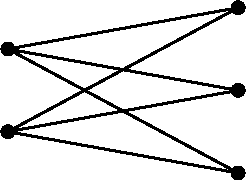
\includegraphics[width=24\unitlength]{K23}}
\cell{12}{21}{c}{$K_{2, 3}$}
\end{picture}%
\hspace*{7mm}%
\begin{picture}(89,62)(-9,-2)
\cell{42}{30}{c}{\includegraphics[width=80\unitlength]{k23new.pdf}}
\cell{43}{-2}{b}{$t$}
\cell{-7}{32}{l}{$\mg{tK_{2,3}}$}
\end{picture}
\caption{The complete bipartite graph $K_{2, 3}$ and its magnitude function
(Example~\ref{eg:k23}).  The singularity is at $\log\sqrt{2} \approx 0.35$.}
\lbl{fig:k23}
\end{figure}

The magnitude function of $K_{2, 3}$ has several striking features: it
is sometimes negative, sometimes greater than the number of points,
sometimes undefined, and sometimes \emph{decreasing} in the scale factor
$t$.  Example~2.2.7 of Leinster~\cite{MMS} gives details.
\end{example}

However, the magnitude function of a finite metric space never behaves
\emph{too} badly.  It can be shown that the magnitude function has only
finitely many singularities (none for subspaces of Euclidean space), that
it is increasing for $t \gg 0$, and that $\mg{tA}$ converges to the
cardinality of $A$ as $t \to \infty$ (Proposition~2.2.6 of
Leinster~\cite{MMS}).  In particular, this last statement implies that the
magnitude function of a space knows its cardinality.

In Example~\ref{eg:k23}, we started from a graph, constructed the metric
space whose points are the vertices and whose distances are shortest
path-lengths, and considered the magnitude of that space.  This is a
construction of general interest, investigated in Leinster~\cite{MG}.  In
this context, we replace the real number $e^{-1}$ in the definition of
magnitude%
% 
\index{magnitude!graph@of graph}%
\index{graph!magnitude of}
% 
by a formal variable $x$.  The magnitude of a graph can then be
expressed as either a rational function or a power series in $x$ with
integer coefficients (Section~2 of~\cite{MG}).  For example, the graphs
\[
\includegraphics[height=2em]{bull.pdf}
\qquad

\includegraphics[height=2em]{tadpole.pdf}
\qquad
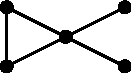
\includegraphics[height=2em]{cricket.pdf}
\]
all have magnitude 
\[
\frac{5 + 5x - 4x^2}{(1 + x)(1 + 2x)}
=
5 - 10x + 16x^2 - 28x^3 + 52x^4 - 100x^5 + \cdots
\]
(Example~4.11 of~\cite{MG}).  The magnitude of a graph shares some
invariance properties with one of the most important graph invariants of
all, the Tutte%
% 
\index{Tutte polynomial}%
\index{polynomial!Tutte}
% 
polynomial.  For instance, it is invariant under Whitney%
% 
\index{Whitney twist}
% 
twists when the points of identification are adjacent.  But it is not a
specialization of the Tutte polynomial: it carries information that the
Tutte polynomial does not.

Graph magnitude satisfies multiplicativity and inclusion-exclusion
principles: 
% 
\begin{align*}
\index{multiplicative!magnitude is}
\mg{G \times H} &
=
\mg{G} \cdot \mg{H},    \\
\index{inclusion-exclusion principle}
\mg{G \cup H}   &
=
\mg{G} + \mg{H} - \mg{G \cap H}
\end{align*}
% 
(where the latter is under quite strict hypotheses), shown as Lemma~3.6
and Theorem~4.9 of Leinster~\cite{MG}.  As such, it has a reasonable claim
to being the graph-theoretic analogue of cardinality.

As additional evidence for this claim, Hepworth%
%
\index{Hepworth, Richard} 
% 
and Willerton~\cite{HeWi}%
%
\index{Willerton, Simon}
% 
constructed a graded homology% 
% 
\index{magnitude!homology}
% 
theory of graphs%
%
\index{graph!magnitude homology of}
% 
whose Euler characteristic is magnitude.  In more detail: since their
homology theory is graded, the Euler characteristic of a graph is not a
single number but a sequence of numbers, which when construed as a power
series is exactly the graph's magnitude.  Thus, their homology theory is a
categorification of magnitude in the same sense that the Khovanov%
%
\index{Khovanov homology}
%
homology of knots and 
links~\cite{Khov} is a categorification of the Jones%
%
\index{Jones polynomial} 
%
polynomial.  It is a finer invariant than magnitude, in that there are
graphs with the same magnitude but different homology groups (Gu~\cite{Gu},
Appendix~A; see also Summers~\cite{Summ}).

Not only the definition of magnitude for graphs, but also some theorems
about it, can be categorified.  For instance, Hepworth and Willerton proved
that the multiplicativity and inclusion-exclusion theorems for magnitude
lift to K\"unneth and Mayer--Vietoris theorems in homology.  In this sense,
known properties of the magnitude of graphs are shadows of functorial
results in homology.

Hepworth and Willerton's idea even works in the full generality of enriched
categories.  That is, the magnitude of an enriched category (a numerical
invariant) can be categorified to a graded homology theory for enriched
categories (an algebraic invariant).  As in the case of graphs,
`categorified' means that the Euler characteristic of the homology theory
is exactly magnitude.  This \demph{magnitude%
%
\index{magnitude!homology}
% 
homology} for enriched categories was defined and developed in work led by
Shulman~\cite{MHECMS}.%
%
\index{Shulman, Michael}
% 
It is a kind of Hochschild homology.

Since metric spaces are a special kind of enriched category, this
construction provides a new homology theory for metric spaces.  It is
genuinely metric rather than topological.  For example, the first magnitude
homology of a closed subset $X$ of $\R^n$ is trivial if and only if $X$ is
convex%
% 
\index{convex!set}
% 
(\cite{MHECMS}, Section~4).  Indeed, all of the magnitude homology groups
of a convex subset of $\R^n$ are trivial, a metric analogue of the
topological fact that the homology of a contractible space is
trivial.  This was proved independently by Kaneta and Yoshinaga
(Corollary~5.3 of~\cite{KaYo}) and by Jubin (Theorem~7.2 of~\cite{Jubi}).
Gomi~\cite{GomiMHG} states a slogan:
%
\index{Gomi, Kiyonori}
% 
\begin{quote}
The more geodesics are unique, the more magnitude homology is trivial.
\end{quote}

Methods for computing the magnitude homology of metric spaces have recently
been developed and applied to calculate specific homology groups.  Gomi
developed spectral sequence techniques and used them to prove results on
the magnitude homology groups of circles (\cite{GomiSFM}, Section~4).
Kaneta and Yoshinaga~\cite{KaYo} showed that while ordinary topological
homology detects the existence of holes, magnitude homology detects the
\emph{diameter} of holes, in a sense made precise in their Theorem~5.7.
Asao proved that if a space contains a closed geodesic then its second
magnitude homology group is nontrivial (Theorem~5.3 of~\cite{Asao}), while
Gomi~\cite{GomiMHG} proved general results on the second and third
magnitude homology groups of metric spaces.

Magnitude homology is not the first homology theory of metric spaces: there
is also persistent%
%
\index{persistent homology}
%
homology, fundamental in the field of topological data analysis.  (For
expository accounts of persistent homology, see Ghrist~\cite{GhriBPT} or
Carlsson~\cite{Carl}.)  Otter~\cite{Otte}%
%
\index{Otter, Nina} 
% 
has proved results relating the two homology theories, introducing for this
purpose a notion of `blurred magnitude homology'; see also Govc and
Hepworth~\cite{GoHe} and Cho~\cite{Cho}.

Finally, Hepworth~\cite{HepwMC} has introduced a theory of magnitude
\emph{cohomology}%
%
\index{magnitude!cohomology}%
\index{Hepworth, Richard}
%
for enriched categories.  It carries a product that formally resembles the
ordinary cup product, but is noncommutative.  For finite metric spaces,
magnitude cohomology is a complete invariant: the cohomology ring
of such a space determines it uniquely up to isometry.



\section{Magnitude in geometry and analysis}
\lbl{sec:mag-geom}


Most metric spaces of geometric interest are not finite.  The general
enriched-categorical concept of magnitude provides no definition of the
magnitude of an infinite metric space.  On the other hand, there are 
several plausible strategies for extending the definition of magnitude from
finite to compact metric spaces.  Meckes~\cite{MeckPDM,MeckMDC}%
% 
\index{Meckes, Mark} 
% 
showed that as long as the space satisfies a certain classical condition,
they all give the same outcome.

The condition is that the space must be of \demph{negative%
%
\index{negative!type} 
% 
type}.  We do not need the original definition here, but Meckes refined old
results of Schoenberg~\cite{SchoMSP} to show that $A$ is of negative type
if and only if the matrix $Z_{tB}$ is positive%
%
\index{positive!definite}
% 
definite for every finite $B \sub A$ and real
$t > 0$ (Theorem~3.3 of~\cite{MeckPDM}).  A great many spaces are of
negative type, including all subspaces of $\R^n$ with the Euclidean or
$\ell^1$ (taxicab) metric, all ultrametric spaces, real and complex
hyperbolic space, and spheres with the geodesic metric.  A list can be
found in Theorem~3.6 of~\cite{MeckPDM}.

The most direct way to state the extended definition of magnitude is as
follows.

\begin{defn}
Let $A$ be a compact metric space of negative type.  The \demph{magnitude}%
% 
\index{magnitude!metric space@of metric space}
% 
of $A$ is
\[
\mg{A} 
= 
\sup \{ \mg{B} \such \text{finite subsets } B \sub A \}
\in 
[0, \infty].
\ntn{magcpt}
\]
\end{defn}

Equivalently, one can choose a sequence $B_1 \sub B_2 \sub \cdots \sub A$
of finite subspaces $B_n$ of $A$ such that $\bigcup B_n$ is dense in $A$,
then put $\mg{A} = \lim_{n \to \infty} \mg{B_n}$.  Equivalently again, one
can define the magnitude of $A$ by the variational formula
% 
\begin{equation}
\lbl{eq:mag-sup}
\mg{A}
=
\sup_\mu
\frac{\mu(A)^2}{\int_A \int_A e^{-d(a, b)} \dee\mu(a) \dee\mu(b)},
\end{equation}
% 
where the supremum is over the finite signed Borel measures $\mu$ on $A$
for which the denominator is nonzero.  

This last characterization is related to yet another formulation.  A
\demph{weight%
%
\index{weight measure} 
% 
measure} on $A$ is a finite signed Borel measure $\mu$ such
that
\[
\int_A e^{-d(a, b)} \dee\mu(b) = 1
\]
for all $a \in A$.  This definition was introduced by Willerton%
%
\index{Willerton, Simon} 
% 
(\cite{WillMSS}, Section~1.1), and is the continuous analogue of the
notion of weighting (Definition~\ref{defn:wtg}).  If $\mu$ is a weight
measure on $A$ then $\mg{A} = \mu(A)$, by Theorem~2.3 of
Meckes~\cite{MeckPDM} or Proposition~5.3.6 of Leinster and
Meckes~\cite{MMSCG}.  However, not every compact metric space of negative
type admits a weight measure.  Most weightings are distributions of a more
general kind, defined in Meckes~\cite{MeckMDC}.%
%
\index{Meckes, Mark}

The equivalence of these and other definitions of magnitude was established
by Meckes~\cite{MeckPDM,MeckMDC},%
%
\index{Meckes, Mark}
% 
using techniques of harmonic and functional analysis.

We now give some examples of compact spaces $A$ and their magnitude
functions $t \mapsto \mg{tA}$.

\begin{example}
\lbl{eg:boxy-line}
The magnitude function of a straight line $[0, \ell]$ of length $\ell$ is
given by 
\[
\mg{t \cdot [0, \ell]} = 1 + \hlf\ell\cdot t.
\]
Several proofs are known, as in Theorem~7 of Leinster and
Willerton~\cite{AMSES},%
%
\index{Willerton, Simon} 
% 
Theorem~2 of Willerton~\cite{WillMSS}, and Proposition~3.2.1 of
Leinster~\cite{MMS}.  The easiest proof uses weight measures.  Let
$\delta_0$ and $\delta_\ell$ denote the point measures at $0$ and $\ell$,
let $\lambda_{[0, \ell]}$ denote Lebesgue measure on $[0, \ell]$, and put
\[
\mu = \hlf(\delta_0 + \lambda_{[0, \ell]} + \delta_\ell).
\]
It is easily verified that $\mu$ is a weight measure on $[0, \ell]$.  Hence
\[
\mg{[0, \ell]} = 1 + \hlf\ell,
\]
and so the magnitude function of $[0, \ell]$ is given by 
\[
\mg{t \cdot [0, \ell]} 
=
1 + \hlf\ell\cdot t.
\]
\end{example}

\begin{example}
\lbl{eg:boxy-boxes}
\index{multiplicative!magnitude is}
% 
Magnitude is multiplicative with respect to the $\ell^1$%
% 
\index{lone geometry@$\ell^1$ geometry} 
% 
product of metric
spaces, that is, the product space with the metric given by adding the
distances in the two factors (Proposition~3.1.4 of Leinster~\cite{MMS}).
This has the following consequence.  Equip $\R^n$ with the $\ell^1$ metric:
\[
d(\vc{x}, \vc{y}) = \sum_{i = 1}^n \mg{x_i - y_i}
\]
($\vc{x}, \vc{y} \in \R^n$).  Then by the previous example, the magnitude
function of a rectangle 
\[
A = [0, \ell] \times [0, m] \sub \R^2
\]
is given by
% 
\begin{align*}
\mg{tA} &
=
\bigl( 1 + \hlf\ell\cdot t \bigr) 
\bigl( 1 + \hlf m\cdot t \bigr)         \\
&
=
1 + \tfrac{1}{2} (\ell + m) \cdot t 
+ \tfrac{1}{4} \ell m \cdot t^2.
\end{align*}
% 
Up to a constant factor, the coefficient of $t^2$ is the area of $A$, the
coefficient of $t$ is the perimeter of $A$, and the constant term is the
Euler characteristic of $A$.  Similar statements apply to
higher-dimensional boxes (Corollary~3.4.3 of Leinster~\cite{MMS}).

For rectangles, and for nonempty convex sets in general, the Euler
characteristic is always $1$.  As such, it may seem pretentious to call the
constant term the `Euler characteristic'.  This usage will be justified
shortly.
\end{example}

To begin to explain the geometric content of magnitude, we need to recall
the concept of intrinsic volumes (Klain and Rota~\cite{KlRo} or Section~4.1
of Schneider~\cite{SchnCBB2}), which with different normalizations are also
known as quermassintegrals or Minkowski functionals.

Consider all reasonable ways of measuring the size of compact convex
subsets of $\R^n$ (which in the present discussion will just be called
\demph{convex}%
%
\index{convex!set}
%
sets).  In the plane $\R^2$, there are at least three ways to measure a
set: take its area, its perimeter, or its Euler characteristic.  These are
$2$-, $1$-, and $0$-dimensional measures, respectively.  The general fact
is that there are $n + 1$ canonical ways of measuring convex subsets of
$\R^n$, which define functions
\[
V_0, \ldots, V_n \from \{\text{convex subsets of } \R^n\} \to \R.
\]
Here $V_i$ is $i$-dimensional, in the sense that $V_i(tA) = t^i V_i(A)$,
and $V_i(A)$\ntn{Vi} is called the $i$th \demph{intrinsic%
% 
\index{intrinsic volume} 
% 
volume} of $A$.

The $i$th intrinsic volume of a convex set $A \sub \R^n$ can be defined as
follows.  Choose at random an $i$-dimensional linear subspace $L$ of
$\R^n$, take the orthogonal projection $\pi_L(A)$ of $A$ onto $L$, then
take its $i$-dimensional volume $\Vol(\pi_L(A))$.  Up to a constant factor,
$V_i(A)$ is the expected value of $\Vol(\pi_L(A))$.

\begin{example}
Let $A$ be a convex subset of $\R^3$. Then $V_0(A)$ is $0$ if $A$ is empty,
and $1$ otherwise. (In both cases, $V_0(A)$ is the Euler%
%
\index{Euler characteristic}
% 
characteristic of $A$.) The first intrinsic volume $V_1(A)$ is proportional
to the expected length of the projection of $A$ onto a random line, and is
called the \demph{mean%
%
\index{mean!width} 
% 
width} of $A$.  The second intrinsic volume $V_2(A)$ is proportional to the
expected area of the projection of $A$ onto a random plane, and it is a theorem
of Cauchy%
% 
\index{Cauchy, Augustin!surface area theorem}%
\index{surface area}
% 
that this is proportional to the surface area of $A$ (Klain and
Rota~\cite{KlRo}, Theorem~5.5.2). Finally, $V_3(A)$ is just the volume of
$A$.
\end{example}

Each of the intrinsic volumes $V_i$ on convex sets is isometry-invariant,
continuous with respect to the Hausdorff metric, and a
\dmph{valuation}: $V_i(\emptyset) = 0$ and 
\[
V_i(A \cup B) = V_i(A) + V_i(B) - V_i(A \cap B)
\]
whenever $A$, $B$ and $A \cup B$ are convex.  The same is, therefore, true
of any linear combination of the intrinsic volumes.  A celebrated theorem
of Hadwiger~\cite{Hadw}%
%
\index{Hadwiger's theorem} 
%
states that such linear combinations are the \emph{only}
isometry-invariant continuous valuations on convex sets.

The intrinsic volumes can be adapted to more general classes of space and
to different geometries.  For instance, we can speak of the volume or
surface area of a sufficiently smooth subset of $\R^n$, and in that
context, the intrinsic volumes are closely related to curvature measures.
(See Section~2.1.1 of Alesker and Fu~\cite{AlFu} for a concise review of
the relationship, Morvan~\cite{Morv} or Gray~\cite{GrayT} for full accounts
of curvature measures, and Alesker~\cite{AlesTVM} for a survey of some more
recent developments.)  The intrinsic volumes can also be defined on any
finite union of convex sets (as in Klain and Rota~\cite{KlRo}).  At these
levels of generality, $V_0$ is no longer trivial; it is the Euler
characteristic. This justifies `Euler%
%
\index{Euler characteristic}
%  
characteristic' as the right name for
$V_0$ even in the case of convex sets.

The next example uses a notion of
intrinsic volume adapted to $\R^n$ with the $\ell^1$ metric.

\begin{example}
\lbl{eg:ell1-cmc}
\index{lone geometry@$\ell^1$ geometry}
% 
Generalizing Example~\ref{eg:boxy-boxes}, let $A \sub \R^n$ be a
\demph{convex\index{convex!body} body}, that is, a convex set with nonempty
interior.  Give $A$ the $\ell^1$ metric.  Then the magnitude function of
$A$ is the polynomial
\[
\mg{tA} 
=
\sum_{i = 0}^n \frac{1}{2^i} V'_i(A) \cdot t^i
\]
(Theorem~5.4.6(2) of Leinster and Meckes~\cite{MMSCG}).  Here
$V'_i(A)$\ntn{ivellone}%
% 
\index{intrinsic volume!lone@$\ell^1$}
% 
is the $\ell^1$ analogue of the $i$th intrinsic volume of $A$, discussed
in~\cite{MMSCG} and in Section~5 of Leinster~\cite{IGON}.  Explicitly, it is
the sum of the $i$-dimensional volumes of the projections of $A$ onto the
$i$-dimensional coordinate subspaces of $\R^n$.  The significance of $2^i$
is that the volume of the unit ball in the $1$-norm on $\R^n$ is $2^i/i!$.

So, for convex bodies in $\R^n$ equipped with the $\ell^1$ metric, the
magnitude function is a polynomial whose degree is the dimension and whose
$i$th coefficient is an $i$-dimensional geometric measure.
\end{example}

For the Euclidean rather than $\ell^1$ metric on $\R^n$, results on
magnitude are harder.  Until 2015, the only convex subset of $\R^n$ whose
magnitude was known was the line segment.  But a significant advance was made
by Barcel\'o and Carbery~\cite{BaCa}, who used PDE methods to prove:

\begin{thm}[Barcel\'o and Carbery]
\lbl{thm:bc}%
\index{Barcel\'o, Juan Antonio}%
\index{Carbery, Anthony}%
% 
Let $n \geq 1$ be odd.  Then:
% 
\begin{enumerate}
\item
\lbl{part:bc-rat}
the magnitude function $t \mapsto \mg{tB^n}$ of the $n$-dimensional unit
Euclidean ball $B^n$ is a rational function over $\Z$ of the radius $t$;%
% 
\index{ball, magnitude of}

\item
\lbl{part:bc-low}
the magnitude functions of $B^1$, $B^3$ and $B^5$ are given by
% 
\begin{align*}
\mg{tB^1}       &
=
1 + t,  \\
\mg{tB^3}       &
=
\frac{1}{3!}(6 + 12t + 6t^2 + t^3),
\\
\mg{tB^5}       &
=
\frac{1}{5!}
\frac{360 + 1080t + 525t^2 + 135t^4 + 18t^5 + t^6}{3 + t}.
\end{align*}
\end{enumerate}
\end{thm}

\begin{proof}
Part~\bref{part:bc-rat} is Theorem~4 of~\cite{BaCa}.  For
part~\bref{part:bc-low}, the formulas for $\mg{tB^3}$ and $\mg{tB^5}$ are
Theorems~2 and~3 of~\cite{BaCa}, and the formula for $\mg{tB^1}$ is
Example~\ref{eg:boxy-line} (not due to Barcel\'o and Carbery, but included
in the statement for completeness).
\end{proof}

In the $\ell^1$ metric on $\R^n$, the magnitude of a ball is a polynomial
in its radius, by Example~\ref{eg:ell1-cmc}.  In the Euclidean metric, it
is no longer a polynomial, but it is the next best thing: a rational
function.  Subsequent work of Willerton~\cite{WillMOBH,WillMOBP}%
%
\index{Willerton, Simon} 
% 
identified exactly which rational function $\mg{tB^n}$ is, in terms of
Bessel%
%
\index{Bessel, Friedrich!polynomials}
%
polynomials and Hankel%
%
\index{Hankel determinants}
%
determinants.

Theorem~\ref{thm:bc} is stated under the hypothesis that $n$ is odd, a
condition imposed in order to put the proof into the realm of differential
rather than pseudodifferential equations.  The magnitude of
even-dimensional balls remains unknown.  Even the 2-dimensional disc $B^2$
has unknown magnitude, although numerical experiments suggest that it is a
certain quadratic polynomial in the radius (Willerton~\cite{WillHCC},
Section~3.2).

Barcel\'o and Carbery also proved a result on general compact sets
(Theorem~1 of~\cite{BaCa}):

\begin{thm}[Barcel\'o and Carbery]
\lbl{thm:bc-vol}%
\index{Barcel\'o, Juan Antonio}%
\index{Carbery, Anthony}%
\index{volume}%
\index{magnitude!determines volume}%
% 
For all $n \geq 1$ and compact $A \sub \R^n$, 
\[
\Vol(A) 
= 
c_n \lim_{t \to \infty} \frac{\mg{tA}}{t^n},
\]
where the constant $c_n$ is $n! \Vol(B^n)$. 
\qed
\end{thm}

The volume of the Euclidean unit ball $B^n$ is given by a standard
classical formula, as in Propositions~6.2.1 and~6.2.2 of Klain and
Rota~\cite{KlRo}, for instance.

By Theorem~\ref{thm:bc-vol}, we can extract the volume of a set from its
magnitude function.  This substantiates the earlier claim that the general
notion of the magnitude of an enriched category encompasses the notion of
volume.

Better still, using methods of global analysis, Gimperlein and Goffeng
proved (Theorem~2(d) of~\cite{GiGo}):

\begin{thm}[Gimperlein and Goffeng]
\lbl{thm:gg}%
\index{Gimperlein, Heiko}%
\index{Goffeng, Magnus}%
\index{magnitude!determines surface area}%
\index{surface area}
% 
Let $n \geq 1$ be odd, and let $A \sub \R^n$ be a bounded set with smooth
boundary such that $A$ is the closure of its interior.  Then the magnitude
function of $A$ has an asymptotic expansion
\[
\mg{tA}
\sim
\sum_{i = 0}^\infty m_i(A) t^{n - i}
\text{ as } t \to \infty,
\]
and up to a known constant factor (depending on $n$ and $i$ but not $A$),
the coefficient $m_i(A)$ is equal to the intrinsic volume $V_{n - i}(A)$
for $i = 0, 1, 2$.  
\qed
\end{thm}

Recent work of Gimperlein, Goffeng and Louca,%
%
\index{Louca, Nikoletta}
%
so far unpublished, removes the restriction that $n$ is odd.

For instance, $m_0(A) = \Vol(A)/n!\Vol(B^n)$ (as in
Theorem~\ref{thm:bc-vol}) and $m_1(A)$ is proportional to the $(n -
1)$-dimensional surface%
%
\index{surface area} 
% 
area of $A$.  In the statement of Theorem~\ref{thm:gg}, the term `intrinsic
volume' has been extended beyond its usual context of convex sets.  A more
precise statement for $i = 2$ is that $m_2(A)$ is proportional to the
integral over $\partial A$ of the mean%
% 
\index{mean!curvature}
% 
curvature of $\partial A$ (which when $A$ is convex is itself proportional
to $V_{n - 2}(A)$).

The magnitude of a metric space does not satisfy the inclusion-exclusion
principle in the strongest conceivable sense, since otherwise, every
$n$-point space would have magnitude $n$.  But Gimperlein and Goffeng
showed that magnitude does satisfy inclusion-exclusion in an asymptotic
sense, using techniques related to the heat equation proof of the
Atiyah--Singer
%
% \index{Atiyah--Singer index theorem}
% 
index theorem and making essential use of \emph{complex} scale factors $t$.
Indeed, for subsets $A$, $B$ and $A \cap B$ of $\R^n$ satisfying the
regularity conditions of Theorem~\ref{thm:gg},
\[
\index{Gimperlein, Heiko}%
\index{Goffeng, Magnus}%
\index{inclusion-exclusion principle!asymptotic}%
\index{magnitude!inclusion-exclusion for}
\mg{t(A \cup B)} + \mg{t(A \cap B)} - \mg{tA} - \mg{tB}
\to 0
\text{ as } t \to \infty
\]
(Remark~3 of~\cite{GiGo}).  This is further evidence for the claim that
magnitude should be regarded as a measure of size.

Finally, we return to diversity.  Meckes%
%
\index{Meckes, Mark}
%  
defined the \demph{maximum%
%
\index{maximum diversity}
% 
diversity} of a compact space $A$ of negative type as
\[
\Dmaxana{A}
=
\sup_\mu
\frac{1}{\int_A \int_A e^{-d(a, b)} \dee\mu(a) \dee\mu(b)},
\]
which is similar to the formula~\eqref{eq:mag-sup} for magnitude, except
that now the supremum runs over only the Borel \emph{probability} measures
$\mu$, as opposed to all signed measures.  (In principle, the formula is
for the maximum diversity of order $2$, but Theorem~7.1 of Leinster and
Roff~\cite{MEMS} implies that the maximum diversity of every order is the same.)
Evidently $\Dmaxana{A} \leq \mg{A}$.

When $A$ is a subset of Euclidean space, $\Dmaxana{A}$ is equal to a
classical quantity, the Bessel%
% 
\index{Bessel, Friedrich!capacity} 
% 
capacity%
% 
\index{capacity}
% 
$C_{(n + 1)/2}(A)$.  As Meckes%
%
\index{Meckes, Mark}
%  
showed, a deep result from the theory of capacities provides an upper bound
on $\mg{A}/\Dmaxana{A}$%
% 
\index{magnitude!maximum diversity@vs.\ maximum diversity}%
\index{maximum diversity!magnitude@vs.\ magnitude}
% 
in terms of $n$ alone (Corollary~6.2 of~\cite{MeckMDC}).
% 
% ; the result used is
% Corollary~3.3.4 of Adams and Hedberg~\cite{AdHe}.  
% 
Thus, magnitude is never very different from this Bessel capacity.

Meckes~\cite{MeckMDC} exploited the connection between magnitude and
maximum diversity to extract information about the dimension of a compact
set $A \sub \R^n$ from its magnitude function.  We have already met some
families of spaces where the magnitude function is a polynomial whose
degree is the dimension (Example~\ref{eg:ell1-cmc}).  But here we allow
non-integer dimensions too.

One of the most important notions of fractional dimension is the
\demph{Minkowski}%
%
\index{dimension}%
\index{Minkowski, Hermann!dimension} 
%
or \demph{box-counting%
%
\index{box-counting dimension} 
% 
dimension} (Section~3.1 of Falconer~\cite{Falc}).  The Minkowski dimension
of a subset of $\R^n$ is always greater than or equal to the Hausdorff
dimension, and equality often holds.  (See p.~43 of~\cite{Falc} for
a summary of how the two dimensions are related.)  For instance, both the
Minkowski and the Hausdorff dimensions of the middle-thirds Cantor set are
$\log 2/\log 3$.
% (Example~3.3 of~\cite{Falc}).  
Write $\Minkdim{A}$\ntn{dimM} for the
Minkowski dimension of a compact set $A \sub \R^n$, if defined.

Roughly speaking, the following result states that $\mg{tA}$ grows like
$t^{\Minkdim{A}}$ when $t$ is large.  Thus, we can can recover the
Minkowski dimension of a space from its magnitude function.  It is due to
Meckes (Corollary~7.4 of~\cite{MeckMDC}).

\begin{thm}[Meckes]
\lbl{thm:mink}%
\index{Meckes, Mark}
\index{magnitude!determines dimension}
% 
Let $A$ be a compact subset of $\R^n$.  Then
\[
\Minkdim{A}
=
\lim_{t \to \infty} \frac{\log \mg{tA}}{\log t},
\]
with one side of the equation defined if and only if the other is.
\qed
\end{thm}

For instance, if $A$ is a subset of $\R^n$ with nonzero volume, then
$\mg{tA}$ grows like $t^n$ when $t$ is large, and by the volume theorem of
Barcel\'o and Carbery, the ratio $\mg{tA}/t^n$ converges to a known
constant times the volume of $A$.  When $A$ is the middle-thirds
Cantor%
%
\index{Cantor set} 
% 
set, $\mg{tA}$ grows like $t^{\log 2/\log 3}$.  (In fact, the magnitude
function of the Cantor set also has a kind of hidden periodicity, as shown
in Section~3 of Leinster and Willerton~\cite{AMSES}.)  For convex subsets
of $\R^n$, more precise statements can be made; Meckes%
%
\index{Meckes, Mark}
% 
bounds the magnitude function of a convex set by a polynomial whose
coefficients are proportional to its intrinsic volumes (\cite{MeckMIV},
Theorem~1). 

Theorem~\ref{thm:mink} demonstrates the usefulness of the concept of
maximum%
% 
\index{maximum diversity!geometry and analysis@in geometry and analysis}
% 
diversity for pure-mathematical purposes in geometry and analysis,
independently of any biological application.

